% Created 2025-04-07 seg 14:49
% Intended LaTeX compiler: lualatex
\documentclass[9 pt]{scrartcl}


\KOMAoptions{
%headings=chapterprefix,
twocolumn=true,
%toc=indenttextentries,
%toc=flat,
twoside=true,
headinclude=true,
footinclude=true
%  captions=topbeside
}
%\usepackage[fontsize=12.3]{scrextend}
\usepackage{fontspec}
\usepackage[T1]{fontenc}
\usepackage[english, portuguese]{babel}
\usepackage{hyperref}
%\usepackage[x11names,svgnames,table]{xcolor}
\usepackage[usenames,dvipsnames]{xcolor}
\defaultfontfeatures{Ligatures=TeX}
%%\setmainfont{Lato}
%%\setmainfont{Charis SIL}
\setmainfont{IBM Plex Serif}
\usepackage{typearea}
\usepackage{lscape}
\usepackage[a4paper]{geometry}
\geometry{a4paper,total={170mm,257mm},left=10mm,right=10mm, top=15mm, bottom=20mm}
\usepackage[english,portuguese]{babel}
\usepackage{amsmath,amsfonts,amsthm,bm}
\usepackage{graphicx}
\usepackage{float,wrapfig}
\usepackage{colortbl}
\usepackage{tabularx}
\usepackage{pst-labo}
\usepackage{setspace}
\usepackage{xfrac}
\usepackage{tikz}
\usepackage{pgfplots}
\pgfplotsset{compat=1.3}
%% Diagraman latex
\usepackage{endiagram}
\usepackage{smartdiagram}
\usepackage[tikz]{bclogo}
\usetikzlibrary{fit,patterns,shadows.blur,shapes,decorations.pathreplacing,decorations.markings,arrows.meta,arrows,positioning,shadows,trees}
\usetikzlibrary{decorations.pathmorphing} %% to chemfig config bond
\usepackage{upgreek}
\usepackage[modules={all}]{chemmacros}
%%\chemsetup{modules={reactions,spectroscopy,thermodynamics,redox,isotopes}}
%%\chemsetup{modules={all}}
\NewChemState\EPot{ symbol=E , subscript-pos=right , superscript=o, pre= , unit=\volt }
%\usepackage[version=4,arrows=pgf-filled]{mhchem}
\usepackage{chemfig,elements,cancel,siunitx}
\NewChemPhase\lqdd{\(\ell\)}
\NewChemPhase\gr{grafite}
\NewChemPhase\reac{reação}
%\setchemfig{fixed length=false, atom sep=2.0em, arrow offset=6pt, scheme debug=false,angle increment=30}
\setchemfig{angle increment=30, atom sep=1.67em, double bond sep=0.67ex, bond style={line width=0.1em}, cram width=0.8ex, cram dash width=0.1em, cram dash sep=0.2em, arrow style={line width=0.067em},  arrow head=-{Triangle}, arrow label sep=1ex, cycle radius coeff=0.75, chemfig style={line width=0.1em}, }
\renewcommand{\CancelColor}{\color{red}}
\usepackage{circuitikz}
\usepackage{mol2chemfig}
\usepackage{subfig,caption}
\captionsetup{font=small, labelfont={bf,sf}}
\usepackage{wrapfig,qrcode}
\usepackage{array,longtable} % ajust colunm table
\newcolumntype{J}{>{\centering\arraybackslash}m{7.5cm}}
\newcolumntype{K}{>{\centering\arraybackslash}m{6.5cm}}
\newcolumntype{L}{>{\centering\arraybackslash}m{5cm}}
\newcolumntype{B}{>{\centering\arraybackslash}m{2.5cm}}
\newcolumntype{N}{>{\centering\arraybackslash}m{1.4cm}}
\usepackage[most]{tcolorbox}
\newcounter{mycounter}
%%% Colobor
%%% Example colorbox
\newtcolorbox{Box2}[2][]{
lower separated=false,
colback=white,
colframe=black,fonttitle=\bfseries,
colbacktitle=black,
coltitle=white,
enhanced, attach boxed title to top left={yshift=-0.1in,xshift=0.15in}, boxed title style={boxrule=0pt,colframe=white,}, title=#2,#1}
%%%%%%%% Cabecalho
\usepackage{framed,amsmath}
\newtcolorbox{mybox}[2][]{
enhanced,title=#2, fonttitle=\sffamily\small,
top=2pt,
bottom=1mm,
boxrule=0.4pt,
coltitle=black,
colback=white,
attach boxed title to top center={yshift=-\tcboxedtitleheight/2,
yshifttext=-\tcboxedtitleheight/2},
boxed title style={
colframe=white,
colback=white,
left=0.2pt,
right=0.2pt},
#1}
\usepackage{tabularray}
%%%%%%
\newtcolorbox{exercisebox}%
{enhanced,breakable,colback=white, colframe=green!15!white,colbacktitle=white!15!pink, coltitle=pink!50!black,left=0pt,right=0mm,top=3mm,bottom=3mm,pad at break=0pt,bottomrule at break=0pt,toprule at break=0pt,borderline={0mm}{0mm}{green!50!white,dashed}, attach boxed title to top center={yshift=-2mm},boxed title style={boxrule=0.4pt},title=Exercícios,}
\usepackage{eso-pic}
\usepackage{etoolbox}
\usepackage{enumitem}
\newcommand\circitem[1]{%
\tikz[baseline=(char.base)]{%https://tex.stackexchange.com/questions/204116/uniform-size-of-circles-around-enumitems
\node[circle,draw=gray, fill=gray!30,
minimum size=1.2em,inner sep=0] (char) {#1};}}
\newcommand\boxitem[1]{%
\tikz[baseline=(char.base)]{%https://tex.stackexchange.com/questions/204116/uniform-size-of-circles-around-enumitems
\node[fill=orange!30,
minimum size=1.2em,inner sep=0] (char) {#1};}}
\newcommand{\dd}[1]{\hspace{2pt}d#1}
\definecolor{color1}{RGB}{0,0,90} % Color of the article title and sections
\definecolor{color2}{RGB}{0,20,20} % Color of the boxes behind the abstract and
\definecolor{cinza}{HTML}{C0C0C0}
%%% Custom Exercios
\usepackage{bohr}
\usepackage{multicol}
\setlength{\columnsep}{1.5cm}
\setlength{\columnseprule}{0.2pt}
\usepackage[no-files]{xsim}
\usepackage{tasks}
\xsimsetup{
goal-print={\pgfmathprintnumber[fixed zerofill,precision=2]{#1}}
}
\newcommand*\circled[2]{\tikz[baseline=(char.base)]{
\node[shape=circle,fill,inner sep=2pt, text=white] (char) {#1};}}
%%%%%-Custom Xsim exercises %%%%%
\DeclareExerciseEnvironmentTemplate{custom}
{%\item[\GetExerciseProperty{counter}]
\Needspace*{0\baselineskip}
\noindent
\circled{\XSIMmixedcase{\GetExerciseProperty{counter}}}~~~%
\noindent
\IfInsideSolutionF{%
\GetExercisePropertyT{points}{ % notice the space
(%
\printgoal{\PropertyValue}
\IfExerciseGoalSingularTF{points}
{%\XSIMtranslate{point}
}
{% \XSIMtranslate{points}
}%
)%
}
}}
{\vspace{\baselineskip}}
%%%%%------- Custom  resposta -------%%%%%%%
\DeclareExerciseEnvironmentTemplate{space}
%{\textbf{\GetExerciseProperty{counter}} }
{\noindent\circled{\XSIMmixedcase{\GetExerciseProperty{counter}}}~~~}
% {\circled{\XSIMmixedcase{\GetExerciseProperty{counter}}}}~~~%
{\qquad}
\newcommand*\answer[1]{%
\XSIMexpandcode{%
\SetExerciseProperty{solution-body}
{\noexpand{\Alph{task}}}}%
#1%
}
%\sisetup{locale=DE}
\xsimsetup{
collect = true,
exercise/within = section,
exercise/template = custom,
exercise/the-counter =  \arabic{exercise},
solution/template= custom ,
%%solution-name = solution,  % used with headings=true
%solution/print=true,
%print-collection/print=both,
%print-solutions/collection=true
%goal-print= {\pgfmathprintnumber[fixed zerofill,precision=1]\num{#1}}
}
\RenewDocumentCommand\printpoints{}{%
\TotalExerciseTypeGoal{exercise}{points}{}{}%
}
\NewTasksEnvironment[label = (\emph{\alph*}), label-width = 12pt]{choice}[\choice]
\newenvironment{questions}{\itemize}{\enditemize}
\everymath{\displaystyle}
\DeclareExerciseHeadingTemplate{solution}{%
\section*{Gabarito}%
}
%\usepackage{filecontents}
\NewTblrTheme{fancy}{
\SetTblrStyle{firsthead}{font=\bfseries}
\SetTblrStyle{firstfoot}{fg=blue2}
\SetTblrStyle{middlefoot}{\itshape}
\SetTblrStyle{caption-tag}{red2}
}

\newcommand{\lh}{\underline{\hspace{1cm}}}
%%\onehalfspacing
\def\professor{Fábio Lima}
\def\aluno{ }
\def\numerochamada{}
\def\disciplina{Química}
%%\def\disciplina{UC III}
%%\def\disciplina{R.A.}
\def\turma{1 Ano }
\def\tipo{{\bfseries Avaliação Bimestral}}
%\def\tipo{\bfseries Simulado }
%\def\tipo{\bfseries Atividade Avaliativa}
\def\bimestre{1 Bimestre}
%\def\escola{E.E. 26 de Agosto}
\def\escola{E.E. José Mamede de Aquino}
%\def\escola{E.E. Joaquim Murtinho}
\def\dataprova{}
\def\PQ{0.84} % Question multiple choice
\def\PQA{2.0} % Question open
\DeclareExerciseCollection{Misturas}
\DeclareExerciseCollection{MisturasOpen}
\DeclareExerciseCollection{TeoriaAtomica}
\DeclareExerciseCollection{TeoriaAtomicaII}
\DeclareExerciseCollection{NumerosQuanticos}
\DeclareExerciseCollection{DistribuicaoEletronica}
\DeclareExerciseCollection{Balan}
\DeclareExerciseCollection{TermoquimicaI}
\DeclareExerciseCollection{RadioatividadeI}
\DeclareExerciseCollection{RadioatividadeIOpen}
\DeclareExerciseCollection{RadioatividadeII}
\DeclareExerciseCollection{RadioatividadeII-P2}
\DeclareExerciseCollection{RadioatividadeIIOpen}
\author{fabio}
\date{\today}
\title{}
\hypersetup{
 pdfauthor={fabio},
 pdftitle={},
 pdfkeywords={},
 pdfsubject={},
 pdfcreator={Emacs 30.1 (Org mode 9.7.11)}, 
 pdflang={English}}
\begin{document}

\selectlanguage{portuguese}
\twocolumn[
%%\input{../Modelos/CabeOficial}
\input{../Modelos/cabenovo}
%\input{../Modelos/mamede}
%\input{../Modelos/26agosto}
%% \input{../Modelos/geral}
%Cada questão vale {\textbf 2,0}

%%\section*{Regime de Progressão Parcial}
%\section*{Atividade}
%\section*{Trabalho}
%%\section*{\disciplina}

%{\bfseries Obrigatório a resolução das questões }

%\input{../Modelos/gabarito}

Total Prova: \printpoints
\smallbreak
\medbreak
\par\vspace{2ex}]

%%%%\input{../Modelos/mamede}


\collectexercises{Misturas}

\begin{exercise}[points=\PQ]
O \textbf{ferro} é um dos componentes da hemoglobina. A falta de ferro na alimentação causa anemia. O processo anêmico pode ser revertido com uma alimentação rica em carnes, verduras, grãos e cereais integrais, sendo, em alguns casos,necessário um suplemento de \textbf{sulfato de ferro (II)}. Nesse contexto, os termos sublinhados no texto acima classificam-se, respectivamente, como:

\begin{choice}
\choice elemento químico e substância composta.
\choice substância simples e substância composta.
\choice mistura homogênea e mistura homogênea.
\choice substância simples e mistura heterogênea.
\choice elemento químico e mistura heterogênea.
\end{choice}
\end{exercise}
\begin{solution}
Letra A
\end{solution}




\begin{exercise}[points=\PQ]
A química é responsável pela melhora em nossa qualidade de vida e está inserida em nosso cotidiano de muitas  formas em substâncias e misturas que constituem diversos materiais. Assinale  a  alternativa  que  apresenta,  respectivamente,  substância  simples,  substância  composta,  mistura homogênea e mistura heterogênea.

\begin{choice}
\choice Água, aço, alumínio, granito.
\choice Alumínio, aço, água, granito.
\choice Alumínio, água, aço, granito.
\choice  Alumínio, água, granito, aço.
\choice  Alumínio, água, aço, granito.
\end{choice}
\end{exercise}
\begin{solution}
LETRA C
\end{solution}



\begin{exercise}[points=\PQ]
Os  peixes,  como  todos  os  animais,  precisam  de  gás  oxigênio  para  realizar  a respiração. Considerando que o meio em que eles vivem é a água, pode-se afirmar que o oxigênio utilizado pelos peixes na respiração se encontra
\begin{choice}
\choice dissolvido na água formando uma solução.
\choice precipitado na água como mistura heterogênea.
\choice na molécula de água.
\choice espalhado pela superfície da água.
\choice no ar.
\end{choice}
\end{exercise}
\begin{solution}
LETRA A
\end{solution}

\begin{exercise}[points=\PQ]
Na preparação do café, a água quente entra em contato com o pó e é separada no coador. As operações envolvidas nessa separação são, respectivamente:
\begin{choice}
\choice destilação e decantação.
\choice  filtração e destilação.
\choice  destilação e coação.
\choice  extração e filtração.
\choice  extração e decantação.
\end{choice}
\end{exercise}
\begin{solution}
LETRA D
\end{solution}

\begin{exercise}[points=\PQ]
Uma mistura formada por gasolina, água, serragem e sal de cozinha pode ser separada nos seus diversos componentes seguindo-se as seguintes etapas:
\begin{choice}
\choice filtração, decantação e destilação.
\choice catação e decantação.
\choice sublimação e destilação.
\choice prensagem e decantação.
\choice destilação e decantação.
\end{choice}
\end{exercise}
\begin{solution}
LETRA A
\end{solution}



\begin{exercise}[points=\PQ]
Numa das etapas do tratamento da água que abastece uma cidade, a água é mantida durante um certo tempo em tanques para que os sólidos em suspensão se depositem no fundo. A essa operação denominamos:
\begin{choice}
\choice filtração.
\choice sedimentação.
\choice sifonação.
\choice centrifugação.
\choice cristalização.
\end{choice}
\end{exercise}
\begin{solution}
LETRA B
\end{solution}




\begin{exercise}[points=\PQ]
Um sólido A está totalmente dissolvido num líquido B. É possível separar o solvente B da mistura por meio de uma:

\begin{choice}
\choice centrifugação.
\choice sifonação.
\choice decantação.
\choice filtração.
\choice destilação.
\end{choice}
\end{exercise}
\begin{solution}
LETRA E
\end{solution}


\begin{exercise}[points=\PQ]
Ao se colocarem hexano (\(d\) = 0,66 g/cm\(^3\)), água (\(d\) = 1 g/cm\(^3\)) e sal (\ch{NaC$\ell$}) em uma vidraria de laboratório conhecida como funil de separação (figura a seguir), assinale o aspecto adequado observado após algum tempo de repouso.

\begin{center}
\begin{center}
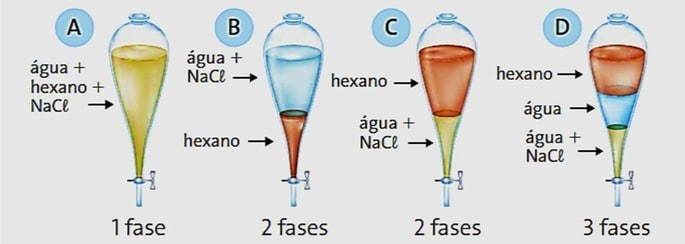
\includegraphics[width=.9\linewidth]{Quimica_Geral/SeparacaoMisturas/funil.jpg}
\end{center}
\end{center}

\begin{choice}(2)
\choice A
\choice B
\choice C
\choice D
\choice nenhuma alternativa
\end{choice}
\end{exercise}
\begin{solution}
LETRA C
\end{solution}


\begin{exercise}[points=\PQ]
Para separar os componentes de uma mistura, foi realizada a seguinte seqüência de operações:

\textbf{aquecimento  =>  adição de água e filtração  =>  evaporação}

Esse procedimento é recomendável para a seguinte mistura:
\begin{choice}
\choice  areia, açúcar e sal
\choice  carvão, areia e açúcar
\choice  ferro, enxofre e álcool
\choice  enxofre, gasolina e ferro
\choice iodo, sal de cozinha e areia
\end{choice}
\end{exercise}
\begin{solution}
LETRA E. A resposta correta é a E. Aquecendo a mistura, separa-se o iodo por sublimação. Adicionando-se água, o sal dissolve-se nesta e separa-se da areia. Uma filtração separa a areia da solução salina. Uma evaporação separa a água do sal.
\end{solution}



\begin{exercise}[points=\PQ]
Para impedir a contaminação microbiana do suprimento de água, deve-se eliminar as emissões de efluentes e, quando necessário, tratá-los com desinfetante. O ácido hipocloroso (\ch{HC$\ell$O}), produzido pela reação entre cloro e água, é um dos compostos mais empregados como desinfetante. Contudo, ele não atua somente como oxidante, mas também como um ativo agente de cloração. A presença de matéria orgânica dissolvida no suprimento de água clorada pode levar à formação de clorofórmio (\ch{CHC$\ell$3}) e outras espécies orgânicas cloradas tóxicas.
Visando eliminar da água o clorofórmio e outras moléculas orgânicas, o tratamento adequado é a:

 {\scriptsize SPIRO, T. G.; STIGLIANI, W. M. {\bfseries Química ambiental}. São Paulo: Pearson, 2009 (adaptado).} 

\begin{choice}
\choice filtração, com o uso de filtros de carvão ativo
\choice fluoretação, pela adição de fluoreto de sódio
\choice coagulação, pela adição de sulfato de alumínio.
\choice correção do pH, pela adição de carbonato de sódio.
\choice floculação, em tanques de concreto com a água em movimento.
\end{choice}
\end{exercise}
\begin{solution}
LETRA A
\end{solution}



\begin{exercise}[points=\PQ]
Assinale a opção que contém a afirmação ERRADA relativa à curva de resfriamento apresentada a seguir.

\begin{tikzpicture}
\begin{axis}[
  line width=1.5pt,
   ticks=none,
   axis x line=bottom,
   axis y line=left,
    xlabel = {\large  Tempo / min},
    ylabel = {\large  Temperatura \textsuperscript{o}C},
    xmin=-10, xmax=100,
    ymin=55, ymax=100,
    xtick={0,20,40,60,80,100},
    ytick={0,20,40,60,80,100},
]

\addplot[
	line width=2pt,
    domain=-10:10, 
    samples=100, 
    color=black,
    ]
    coordinates {
    (0,100)(15,80)(25,80)(30,80)(40,80)(60,80)(80,60)
    };
\end{axis}
\end{tikzpicture}

\begin{choice}
\choice A curva pode representar o resfriamento de uma mistura eutética.
\choice  A curva pode representar o resfriamento de uma substância sólida, que apresenta uma única forma cristalina.
\choice  A curva pode representar o resfriamento de uma mistura azeotrópica.
\choice A curva pode representar o resfriamento de um líquido constituído por uma substância pura.
\choice  A curva pode representar o resfriamento de uma mistura líquida de duas substâncias que são completamente miscíveis no estado sólido.
\end{choice}
\end{exercise}
\begin{solution}
LETRA B
\end{solution}


\begin{exercise}[points=\PQ]
Entre as substâncias usadas para o tratamento de água está o sulfato de alumínio que, em meio alcalino, forma partículas em suspensão na água, às quais as impurezas presentes no meio se aderem.

O método de separação comumente usado para retirar o sulfato de alumínio com as impurezas aderidas é a:
\begin{choice}(2)
\choice flotação.
\choice levigação.
\choice  ventilação.
\choice  peneiração.
\choice  centrifugação.
\end{choice}
\end{exercise}
\begin{solution}
LETRA A
\end{solution}


\begin{exercise}[points=\PQ]
Um grupo de pesquisadores desenvolveu um método simples, barato e eficaz de remoção de petróleo contaminante na água, que utiliza um plástico produzido a partir do líquido da castanha-de-caju (LCC).

A composição química do LCC é muito parecida com a do petróleo e suas moléculas, por suas características, interagem formando agregados com o petróleo.

Para retirar os agregados da água, os pesquisadores misturam ao LCC nanopartículas magnéticas.

KIFFER, D. \emph{Novo método para remoção de petróleo usa óleo de mamona e castanha-de-caju}.
Disponível em: www.faperj.br. Acesso em: 31 jul. 2012 (adaptado).

Essa técnica considera dois processos de separação de misturas, sendo eles, respectivamente:
\begin{choice}
\choice flotação e decantação.
\choice decomposição e centrifugação.
\choice floculação e separação magnética.
\choice destilação fracionada e peneiração.
\choice dissolução fracionada e magnetização.
\end{choice}
\end{exercise}
\begin{solution}
LETRA C
\end{solution}


\collectexercisesstop{Misturas}

\collectexercises{MisturasOpen}

\begin{exercise}[points=1.0]
Separação de misturas é uma operação muito comum no setor de petróleo e combustíveis. Diversos métodos são aplicados para atender a essa necessidade. Sabendo-se que a água e o álcool são miscíveis e o óleo imiscível nestes e que o álcool tem o menor e o óleo o maior ponto de ebulição, quais os métodos adequados para separar essas três substâncias? Explique.

\blank[width=9.\linewidth,linespread=1.5]{}
\end{exercise}




\begin{exercise}[points=1.0]
Responder à questão numerando corretamente a coluna que contém exemplos de sistemas, de acordo com a que apresenta a classificação dos mesmos.

\begin{center}
\begin{tabular}{ll}
1.  elemento    químico & (\quad) fluoreto de sódio\\
2.  substância  simples & (\quad ) gás oxigênio\\
3.  substância  composta & (\quad ) água do mar filtrada\\
4.  mistura     homogênea & (\quad ) limonada com gelo\\
5.  mistura     heterogênea & (\quad ) Vinho\\
\end{tabular}
\end{center}
\end{exercise}




\collectexercisesstop{MisturasOpen}
\printrandomexercises[collection=Misturas]{7}



\collectexercises{TeoriaAtomica}

\begin{exercise}[points=\PQ]
O átomo é a menor partícula que identifica um elemento químico. Ele possui duas partes, a saber: uma delas é o núcleo, constituído por prótons e nêutrons, e a outra é a região externa – a eletrosfera-, por onde circulam os elétrons. Alguns experimentos permitiram a descoberta das características das partículas constituintes do átomo.

Em relação a essas características, indique a alternativa correta.

\begin{choice}
\choice prótons e elétrons possuem massas iguais e cargas elétricas de sinais opostos.
\choice  entre as partículas atômicas, os elétrons têm maior massa e ocupam maior volume no átomo.
\choice entre as partículas atômicas, os prótons e os nêutrons têm maior massa e ocupam maior volume no átomo.
\choice entre as partículas atômicas, os prótons e os nêutrons têm mais massa, mas ocupam um volume muito pequeno em relação ao volume total do átomo.
\choice As partículas não possuem massa.
\end{choice}
\end{exercise}
\begin{solution}
LETRA D
\end{solution}


\begin{exercise}[points=\PQ]
Os estudos realizados por Rutherford mostraram que o átomo deveria ser constituído por um núcleo positivo com elétrons girando ao seu redor. Os elétrons foram inicialmente levados em consideração no modelo atômico proposto pelo seguinte pesquisador.

\begin{choice}
\choice  Niels Borh
\choice J. J. Thomson
\choice John Dalton.
\choice  Werner Heisenberg
\choice Max Planck
\end{choice}
\end{exercise}
\begin{solution}
LETRA B
\end{solution}


\begin{exercise}[points=\PQ]
Comemora-se, neste ano de 2011, o centenário do modelo atômico proposto pelo
físico neozelandês Ernest Rutherford (1871-1937), prêmio Nobel da Química em 1908. Em 1911,Rutherford, bombardeou uma finíssima lâmina de ouro com partículas alfa, oriundas de uma amostra contendo o elemento químico polônio. De acordo com o seu experimento, Rutherford concluiu que

\begin{choice}
\choice o átomo é uma partícula maciça e indestrutível.
\choice os elétrons estão mergulhados em uma massa homogênea de carga positiva.
\choice a maioria das partículas alfa sofria um desvio ao atravessar a lâmina de ouro.
\choice existem, no átomo, mais espaços vazios do que preenchidos.
\choice o átomo é pudim de passas incrustado de carga negativa em um esfera positiva
\end{choice}
\end{exercise}
\begin{solution}
LETRA C
\end{solution}



\begin{exercise}[points=\PQ]
O filme \emph{"Homem de Ferro 2"} retrata a jornada de Tony Stark para substituir o metal paládio, que faz parte do reator de seu peito, por um metal atóxico. Após interpretar informações deixadas por seu pai, Tony projeta um holograma do potencial substituto, cuja imagem se assemelha à figura abaixo

\begin{center}
\tikzset{every picture/.style={line width=0.75pt}} %set default line width to 0.75pt        

\begin{tikzpicture}[x=0.75pt,y=0.75pt,yscale=-1,xscale=1]
%uncomment if require: \path (0,300); %set diagram left start at 0, and has height of 300

%Shape: Circle [id:dp5016060929568149] 
\draw   (108,184) .. controls (108,153.07) and (133.07,128) .. (164,128) .. controls (194.93,128) and (220,153.07) .. (220,184) .. controls (220,214.93) and (194.93,240) .. (164,240) .. controls (133.07,240) and (108,214.93) .. (108,184) -- cycle ;
%Shape: Circle [id:dp7913851496733558] 
\draw  [color={rgb, 255:red, 8; green, 8; blue, 8 }  ,draw opacity=1 ][fill={rgb, 255:red, 10; green, 10; blue, 10 }  ,fill opacity=1 ] (146.5,184) .. controls (146.5,174.34) and (154.34,166.5) .. (164,166.5) .. controls (173.66,166.5) and (181.5,174.34) .. (181.5,184) .. controls (181.5,193.66) and (173.66,201.5) .. (164,201.5) .. controls (154.34,201.5) and (146.5,193.66) .. (146.5,184) -- cycle ;
\end{tikzpicture}

\end{center}
\vspace{2cm}

Essa imagem é uma representação do modelo de
\begin{choice}
\choice Rutherford.
\choice Thomson.
\choice Dalton.
\choice Howard Stark  
\choice Frezza
\end{choice}
\end{exercise}
\begin{solution}
LETRA A
\end{solution}


\begin{exercise}[points=\PQ]
Para o valor do número quântico principal \textbf{n} igual a 4, os tipos de orbitais que podem existir na configuração eletrônica de um átomo podem ser:
\begin{choice}
\choice  s, p, d, f.
\choice  somente s, p, d.
\choice  somente p e f.
\choice somente s e p.
\choice somente d e f
\end{choice}
\end{exercise}
\begin{solution}
LETRA A
\end{solution}



\begin{exercise}[points=\PQ]
O bombardeamento da folha de ouro com partículas alfa, no experimento de Rutherford, mostra que algumas dessas partículas sofrem desvio acentuado do seu trajeto, o que é devido ao fato de que as partículas alfa:
\begin{choice}(1)
\choice Chocam-se com as moléculas de ouro.
\choice Têm carga negativa e são repelidas pelo núcleo.
\choice São muito lentas e qualquer obstáculo as desvia.
\choice Têm carga positiva e são repelidas pelo núcleo.
\choice Não podem atravessar a lâmina de ouro.
\end{choice}
\end{exercise}
\begin{solution}
LETRA D
\end{solution}



\begin{exercise}[points=\PQ]
A experiência de Rutherford, que foi, na verdade, realizada por dois de seus orientados, Hans Geiger e Ernest Marsden, serviu para refutar especialmente o modelo atômico:
\begin{choice}(2)
\choice de Bohr.
\choice de Thomson.
\choice planetário.
\choice quântico.
\choice de Dalton.
\end{choice}
\end{exercise}
\begin{solution}
LETRA B
\end{solution}

\begin{exercise}[points=\PQ]
Assinale a afirmativa que descreve \textbf{ADEQUADAMENTE} a teoria atômica de Dalton. Toda matéria é constituída de átomos:
\begin{choice}
\choice os quais são formados por partículas positivas e negativas.
\choice os quais são formados por um núcleo positivo e por elétrons que gravitam livremente em torno desse núcleo.
\choice os quais são formados por um núcleo positivo e por elétrons que gravitam em diferentes camadas eletrônicas.
\choice e todos os átomos de um mesmo elemento são idênticos.
\choice Nenhuma das alternativas acima.
\end{choice}
\end{exercise}
\begin{solution}
LETRA D
\end{solution}



\begin{exercise}[points=\PQ]
Quem introduziu pela primeira vez o princípio da incerteza?

\begin{choice}(2)
\choice Pauli
\choice De Broglie
\choice Dirac
\choice Schrödinger
\choice Heisenberg
\end{choice}
\end{exercise}
\begin{solution}
Letra E
\end{solution}



\begin{exercise}[points=\PQ]
Qual das alternativas a seguir \textbf{NÃO} é uma limitação do modelo de Bohr do átomo?

\begin{choice}
\choice Os elétrons se movem ao redor do núcleo em órbitas circulares e planas.
\choice Os elétrons são considerados apenas como partículas e não como ondas.
\choice É possível determinar com precisão a posição e o momento de um elétron simultaneamente.
\choice Os elétrons dentro dos átomos só podem ocupar níveis de energia quantizados.
\choice Ele explica apenas o espectro de emissão de linha do átomo de hidrogênio.
\end{choice}
\end{exercise}
\begin{solution}
C
\end{solution}



\begin{exercise}[points=\PQ]
Qual das seguintes afirmações é \textbf{verdadeira} sobre um elétron?

\begin{choice}
\choice Está localizado mais longe do núcleo quando absorve energia.
\choice Absorve energia quando se move de um estado de maior energia para o estado fundamental.
\choice Está localizado no núcleo quando absorve energia.
\choice Está localizado mais perto do núcleo quando absorve energia.
\choice Quando libera energia se move para um estado de maior energia
\end{choice}
\end{exercise}
\begin{solution}
E
\end{solution}



\begin{exercise}[points=\PQ]
Qual das alternativas a seguir melhor descreve um \textbf{elétron}?
\begin{choice}
\choice Uma partícula carregada positivamente com uma massa muito menor que a do núcleo
\choice Uma partícula carregada negativamente com uma massa muito menor que a do núcleo
\choice Uma partícula carregada positivamente com uma massa muito maior que a do núcleo
\choice Uma partícula carregada negativamente com uma massa muito maior que a do núcleo
\choice Partícula neutra com massa igual à do núcleo.
\end{choice}
\end{exercise}
\begin{solution}
D
\end{solution}



\begin{exercise}[points=\PQ]
Qual das alternativas a seguir melhor define o \textbf{número atômico} ?

\begin{choice}
\choice O número total de prótons e nêutrons no núcleo de um átomo
\choice O número de prótons no núcleo de um átomo
\choice O número de nêutrons no núcleo de um átomo
\choice O número total de prótons, nêutrons e elétrons em um átomo
\choice O número de elétrons no núcleo de um átomo
\end{choice}
\end{exercise}
\begin{solution}
B
\end{solution}





\begin{exercise}[points=\PQ]
Uma moda recente entre as crianças é colecionar figurinhas que brilham no escuro. As figuras apresentam em sua constituição, a substância sulfeto de zinco. O fenômeno ocorre porque alguns elétrons que compõem os átomos de zinco absorvem energia luminosa, saltando para níveis de energia mais externos. No escuro, esses elétrons retornam aos seus níveis de origem, liberando energia luminosa e fazendo a figurinha brilhar.

Essa característica pode ser explicada considerando o modelo atômico proposto por:

\begin{choice}
\choice Bohr.
\choice Rutherford.
\choice Lavoisier.
\choice Thomson.
\choice Dalton.
\end{choice}
\end{exercise}
\begin{solution}
A
\end{solution}



\begin{exercise}[points=\PQ]
Qual das imagens a seguir representa melhor o modelo atômico do pudim de passas de Thomson?


\begin{choice}(1)
\choice \resizebox{.2\textwidth}{!}{%
\begin{circuitikz}
\tikzstyle{every node}=[font=\LARGE]
\draw  (2,12.25) circle (1.75cm);
\draw  (1,13.25) circle (0.25cm);
\draw  (2,13.25) circle (0.25cm);
\draw  (1.5,12) circle (0.25cm);
\draw  (2.75,12.25) circle (0.25cm);
\draw  (2.25,11.25) circle (0.25cm);
\node [font=\LARGE] at (1.5,11) {+};
\node [font=\LARGE] at (3,13) {+};
\node [font=\LARGE] at (2.5,11.5) {+};
\node [font=\LARGE] at (0.75,12.25) {+};
\node [font=\LARGE] at (2,12.5) {+};
\node [font=\LARGE] at (2.25,11.25) {-};
\node [font=\LARGE] at (2.75,12.25) {-};
\node [font=\LARGE] at (2,13.25) {-};
\node [font=\LARGE] at (1,13.25) {-};
\node [font=\LARGE] at (1.5,12) {-};
\end{circuitikz}
}%


\choice \resizebox{.2\textwidth}{!}{%
\begin{circuitikz}
\tikzstyle{every node}=[font=\LARGE]
\draw [fill={rgb, 255:red, 122; green, 119; blue, 119 }  ,fill opacity=1 ] (2,12.25) circle (1.75cm);
\end{circuitikz}
}%







\choice 	\resizebox{0.2\textwidth}{!}{%
		\begin{circuitikz}
			\tikzstyle{every node}=[font=\LARGE]
			\draw  (2,12.25) circle (1.75cm);
			\draw  (0.75,12.25) circle (0.25cm) node {\LARGE -} ;
			\draw  (1.5,13.25) circle (0.25cm);
			\draw  (3,12.5) circle (0.25cm);
			\draw  (2.25,11) circle (0.25cm) node {\LARGE -} ;
			\draw  (2,12.25) circle (0.5cm);
			\node [font=\huge] at (2,12.25) {+};
			\node [font=\large] at (1.5,13.25) {-};
			\node [font=\large] at (3,12.5) {-};
		\end{circuitikz}
	}%

\choice \resizebox{.2\textwidth}{!}{%
\begin{circuitikz}
\tikzstyle{every node}=[font=\LARGE]
\draw  (2,12.25) circle (1.75cm);
\draw [ fill={rgb,255:red,192; green,191; blue,188} ] (2,10.5) circle (0.25cm) node {\LARGE -} ;
\draw [ fill={rgb,255:red,192; green,191; blue,188} ] (0.25,12) circle (0.25cm) node {\LARGE -} ;
\draw [ fill={rgb,255:red,192; green,191; blue,188} ] (2,14) circle (0.25cm) node {\LARGE -} ;
\draw [ fill={rgb,255:red,192; green,191; blue,188} ] (3.75,12) circle (0.25cm) node {\LARGE -} ;
\draw  (2,12.25) circle (0.5cm) node {\LARGE +} ;
\end{circuitikz}
}%



\choice \resizebox{.2\textwidth}{!}{%
\begin{circuitikz}
\tikzstyle{every node}=[font=\LARGE]
\draw  (2,12.25) circle (1.75cm);
\draw  (2,12.25) circle (0.5cm) node {\LARGE +} ;
\end{circuitikz}
}%

\end{choice}
\end{exercise}




\begin{exercise}[points=\PQ]
Qual químico descobriu que os elétrons existem em níveis de energia fixos?
\begin{choice}
\choice Bohr
\choice Thomson
\choice Dalton
\choice Geiger e Marsden
\choice Rutherford
\end{choice}
\end{exercise}
\begin{solution}
A
\end{solution}


\begin{exercise}[points=\PQ]
Na experiência de Geiger-Marsden supervisionada por Ernest Rutherford (conhecida como a experiência da folha de ouro de Rutherford), que tipo de partícula foi dispersada por uma folha de ouro, provando que os átomos contêm um núcleo denso?

\begin{choice}
\choice Raios gama
\choice Nêutrons
\choice Partículas \(\upbeta^+\)
\choice Partículas \(\upbeta^-\)
\choice Partículas \(\upalpha\)
\end{choice}
\end{exercise}

\begin{solution}
E
\end{solution}

\begin{exercise}[points=\PQ]
Qual é a principal força atrativa entre partículas no núcleo de um átomo?

\begin{choice}
\choice Gravidade
\choice Forca eletrostática
\choice Força nuclear forte
\choice Força nuclear fraca
\choice Força eletromagnética
\end{choice}
\end{exercise}
\begin{solution}
C
\end{solution}

\begin{exercise}[points=\PQ]
Que passo em frente, a partir do modelo atômico das orbitais de Bohr, foi dado por Schrödinger no seu modelo da nuvem eletrónica?

\begin{choice}
\choice O núcleo contém partículas com massa mas sem carga.
\choice Os elétrons ocupam níveis de energia com raios fixos.
\choice O núcleo contém partículas com massa e carga positiva.
\choice Os elétrons movem-se dentro de uma esfera positivamente carregada.
\choice Os elétrons estão dispersos no espaço.
\end{choice}
\end{exercise}
\begin{solution}
E
\end{solution}


\begin{exercise}[points=\PQ]
Em que é que o modelo atômico de Thomson é diferentes do modelo atômico de Dalton?

\begin{choice}
\choice O modelo atômico de Thomson inclui partículas com carga negativa conhecidas como elétrons
\choice O modelo atômico de Thomson mostra elétrons a ocupar os vértices de um cubo.
\choice O modelo atômico de Thomson inclui partículas com carga positiva conhecidas como prótons
\choice O modelo atômico de Thomson descreve elétrons a orbitar um núcleo central.
\choice O modelo atômico de Thomson mostra elétrons a ocupar diferentes níveis de energia.
\end{choice}
\end{exercise}
\begin{solution}
A
\end{solution}



\collectexercisesstop{TeoriaAtomica}
\collectexercises{TeoriaAtomicaII}



\begin{exercise}[points=\PQ]
\textbf{(UPE)} Observe a charge a seguir.

\begin{figure}[htbp]
\centering
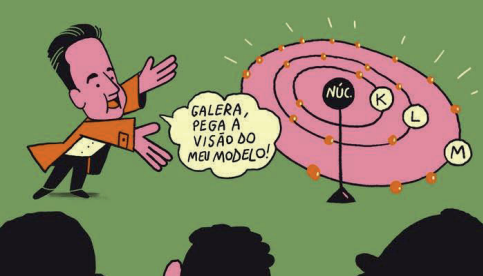
\includegraphics[width=.9\linewidth]{Quimica_Geral/TeoriaAtomica/charge.png}
\caption{}
\end{figure}

Com base no modelo atômico apresentado na imagem, quem é a personagem representada?

\begin{choice}(2)
\choice Albert Einstein
\choice John Dalton
\choice Ernest Rutherford
\choice George Paget Thomson
\choice Niels Bohr
\end{choice}
\end{exercise}
\begin{solution}
E
\end{solution}




\begin{exercise}[points=\PQ]
O desenvolvimento dos modelos atômicos é um excelente exemplo de como os modelos científicos se desenrolam e são, constantemente, revisados. O modelo atual foi desenvolvido a partir de estudos de diferentes pesquisadores e séries de experimentos.

Sobre os modelos atômicos, assinale a alternativa correta.

\begin{choice}


\choice Segundo Bohr, os elétrons circulam ao redor do núcleo em determinadas órbitas de energia. 
\choice Segundo Dalton, átomos são esferas constituídas de partículas subâtomicas.
\choice J. J. Thomson propôs a existência de partículas positivas (prótons) em uma esfera negativa.
\choice Segundo Rutherford, o átomo tem o núcleo positivo mais leve, com elétrons pesados ao redor.
\choice Segundo o modelo de subníveis de energia, um átomo com Z=22 tem configuração 1s\textsuperscript{2} 2s\textsuperscript{2} 2p\textsuperscript{6} 3s\textsuperscript{2} 3d$^{10}$.
\end{choice}
\end{exercise}


\begin{exercise}
Analogias são muito usuais como estratégias para abordar conhecimentos científicos, pois possuem o potencial de apresentar ideias mais complexas (domínio-alvo) a partir de ideias mais simples (domínio análogo). Contudo, algumas vezes, existe o uso abusivo, como na tirinha a seguir:

\begin{center}
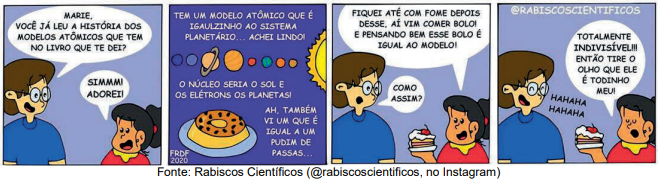
\includegraphics[width=.9\linewidth]{Quimica_Geral/TeoriaAtomica/charge2.png}
\end{center}

Mesmo com o uso abusivo das analogias, podemos reconhecer, na ordem em que aparecem, os modelos atômicos propostos por

\begin{choice}
\choice Dalton, Thomson, Bohr.
\choice Modelo Quântico, Dalton e Rutherford.
\choice Rutherford, Bohr e Thomson. 
\choice Rutherford, Thomson e Dalton.
\choice Dalton, Modelo Quântico e Bohr.
\end{choice}
\end{exercise}


\begin{exercise}[points=\PQ]
\textbf{(CESMAC)} John Dalton, químico inglês, nascido em 1766, é um dos principais pesquisadores relacionados à teoria atômica, tendo descrito o primeiro modelo atômico conhecido.

Acerca do modelo atômico de Dalton, assinale a alternativa \textbf{incorreta}.

\begin{choice}
\choice Os elementos são feitos de partículas extremamente pequenas chamadas átomos.
\choice Os átomos de um determinado elemento são idênticos em tamanho, massa e outras propriedades; átomos de diferentes elementos diferem em tamanho, em massa e em outras propriedades.
\choice Nas reações químicas, os átomos são combinados, separados ou reorganizados.
\choice Átomos de diferentes elementos combinam-se em proporções simples de número inteiro para formar compostos químicos.
\choice Os átomos podem ser subdivididos, criados ou destruídos.
\end{choice}
\end{exercise}


\begin{exercise}[points=\PQ]
A tirinha a seguir apresenta uma crítica à forma de abordagem do estudo dos modelos atômicos:

\begin{center}
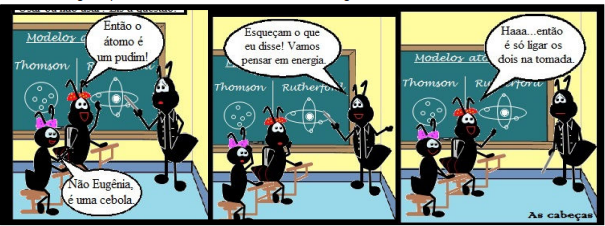
\includegraphics[width=.9\linewidth]{Quimica_Geral/TeoriaAtomica/charge3.png}
\end{center}

A analogia estabelecida na charge entre o modelo atômico de Thomson e um “pudim” é comumente usada, pois a característica do modelo é:

\begin{choice}(1)
\choice Núcleo central de carga positiva e elétrons em órbitas com valores de energia definidos.

\choice Elétron, de carga negativa, incrustado em uma esfera de carga positiva distribuída homogeneamente por toda a esfera. 

\choice Átomos maciços e indivisíveis, não apresentando carga, e formadores de todas as substâncias químicas. 

\choice Elétron como partícula-onda com trajetória desconhecida, presente em nuvem eletrônica, ocupando o orbital.
\end{choice}
\end{exercise}



\begin{exercise}[points=\PQ]
Uma forma de determinar a extensão de uma fratura em um osso do corpo é por meio do uso do equipamento de Raios X. Para que essa tecnologia e outros avanços tecnológicos pudessem ser utilizados, um grande passo teve de ser dado pelos cientistas: a concepção científica do modelo atômico. Sobre o modelo atômico proposto, associe as afirmações da coluna 1, com seus respectivos responsáveis, na coluna 2.



\textbf{Coluna 1}



\begin{enumerate}
\item Toda a matéria é formada por átomos, partículas esféricas, maciças, indivisíveis e indestrutíveis.
\item Elaborou um modelo de átomo constituído por uma esfera maciça, de carga elétrica positiva, que continha “corpúsculos” de carga negativa (elétrons) nela dispersos.
\item O átomo seria constituído por duas regiões: uma central, chamada núcleo, e uma periférica, chamada de eletrosfera.
\item Os elétrons ocupam determinados níveis de energia ou camadas eletrônicas.
\end{enumerate}



\textbf{Coluna 2}



( ) Rutherford-Bohr

( ) Rutherford

( ) Dalton

( ) Thomson



A sequência correta de preenchimento dos parênteses da coluna 2, de cima para baixo, é

\begin{choice}
\choice 2 – 3 – 1 – 4. 
\choice 3 – 2 – 1 – 4.
\choice 4 – 3 – 1 – 2. 
\choice 3 – 4 – 1 – 2. 
\choice 4 – 2 – 1 – 3.
\end{choice}
\end{exercise}






\begin{exercise}[points=\PQ]
Na Inglaterra por volta de 1900, uma série de experimentos realizados por cientistas, como Sir Joseph John Thompson (1856-1940) e Ernest Rutherford (1871-1937), estabeleceu um modelo do átomo que serviu de base à teoria atômica. Atualmente, sabe-se que três partículas subatômicas são os constituintes de todos os átomos: próton, nêutrons e elétrons. Desta forma, o átomo constituído por 17 prótons, 18 nêutrons e 17 elétrons possui número atômico e número de massa, sequencialmente, igual a: 

\begin{choice}(2)
\choice 17 e 18 
\choice 34 e 52 
\choice 17 e 17 
\choice 17 e 35
\choice 35 e 17 
\end{choice}
\end{exercise}



\begin{exercise}[points=\PQ]
Os cientistas que trabalharam no estudo do átomo foram fundamentais para que a humanidade pudesse avançar no seu caminho de desvendar os mistérios da composição da matéria. Sabe-se que ainda há muito para se descobrir, por isso a atomística e a física de partículas subatômicas ainda são áreas extremamente fascinantes.



Assinale abaixo a alternativa que relaciona corretamente o cientista e a principal inovação que seu modelo atômico trouxe na compreensão da natureza íntima da matéria.

\begin{choice}
\choice Erwin Schroedinger e a existência da dualidade onda-partícula do elétron.
\choice eErnest Rutherford e a existência dos quarks.
\choice Joseph Thomson e a existência de um núcleo atômico pequeno e muito denso.
\choice John Dalton e a existência de cargas elétricas opostas espalhadas no átomo.
\choice  Niels Bohr e a existência de níveis energéticos quantizados na eletrosfera.
\end{choice}
\end{exercise}


\begin{exercise}[points=\PQ]
\textbf{(UNESP)} Na evolução dos modelos atômicos, a principal contribuição introduzida pelo modelo de Bohr foi:

\begin{choice}
\choice a indivisibilidade do átomo.
\choice  a existência de nêutrons.
\choice a natureza elétrica da matéria.
\choice a quantização de energia das órbitas eletrônicas.
\choice a maior parte da massa do átomo está no núcleo.
\end{choice}
\end{exercise}



\begin{exercise}[points=\PQ]
Analise as afirmações abaixo, sobre os modelos atômicos.
\begin{enumerate}
\item \textbf{John Dalton:} Afirmava que toda a matéria é formada por partícula extremamente pequena, e é indivisível.
\item \textbf{Thomson:} Formulou a teoria segundo a qual o átomo é uma esfera positiva que, para tornar-se neutra, apresenta elétrons (partículas negativas) presos em sua superfície.
\item \textbf{Erwin Schrödinger:} O físico propôs a teoria que demonstra a probabilidade de se encontrar o elétron em torno do núcleo (orbital).
\end{enumerate}


Assinale a alternativa correta em relação a essas afirmativas.

\begin{choice}
\choice O modelo formulado por John Dalton ficou conhecido como "pudim de passas".
\choice O modelo proposto por Erwin Schrödinger é utilizado até hoje.
\choice John Dalton provou que o átomo é uma partícula dividida em prótons elétrons e nêutrons.
\choice Thomson foi o autor da frase O átomo é uma partícula formada apenas por uma única carga .
\choice Pertence ao físico Erwin Schödinger a expressão pudim de passas , que se refere à estrutura atômica da matéria.
\end{choice}
\end{exercise}




\begin{exercise}[points=\PQ]
\textbf{(UNIPAM)} Ainda antes de Cristo, os filósofos especulavam sobre a natureza da matéria da qual o universo era feito, com o intuito de explicar a sua constituição. Já os séculos XVII e XVIIIcaracterizaram se, na história da química, pela aquisição de um grande número de informações obtidas experimentalmente. Nessa época deu-se uma certa preferência aos processos químicos e, como consequência, o conhecimento químico cresceu em quantidade e em qualidade. No final desse período, inúmeros fatos químicos floresceram. A evolução histórica do modelo atômico encontra-se resumida na figura a seguir.

\begin{center}
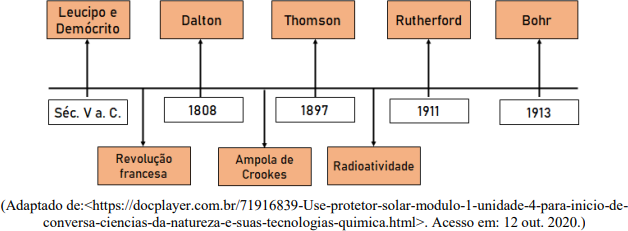
\includegraphics[width=.9\linewidth]{Quimica_Geral/TeoriaAtomica/evolucao.png}
\end{center}

Assinale a alternativa \textbf{CORRETA} acerca da teoria atômica.

\begin{choice}
\choice Leucipo e Demócrito foram os primeiros cientistas a formalizar, do ponto de vista quantitativo, a existência dos átomos.

\choice  Bohr mostrou que o átomo consiste em um minúsculo núcleo que contém toda a carga positiva e quase toda a massa do átomo.

\choice Dalton dispunha de dados experimentais que possibilitaram afirmar que átomos de elementos diferentes possuem massas diferentes.

\choice Rutherford desenvolveu um modelo atômico segundo o qual, quando o elétron passa de uma órbita para outra, emite ou absorve uma quantidade de energia.

\choice Nenhuma das alternativas
\end{choice}
\end{exercise}







\collectexercisesstop{TeoriaAtomicaII}
\collectexercises{NumerosQuanticos}

\begin{exercise}[points=\PQ]
Qual é o conjunto dos quatro números quânticos que caracteriza o elétron mais energético do  $_{35}$Br?
\begin{choice}
\choice n = 3, \(l\) = 2, m\textsubscript{s} = +2, s = +1/2.
\choice n = 4, \(l\) = 0, m\textsubscript{s} = 0, s = +1/2.
\choice n = 3, \(l\) = 1, m\textsubscript{s} = +2, s = +1/2.
\choice n = 4, \(l\) = 1, m\textsubscript{s} = 0, s = +1/2.
\choice n = 4, \(l\) = 3, m\textsubscript{s} = +2, s = +1/2. 
\end{choice}
\end{exercise}
\begin{solution}
D
\end{solution}



\begin{exercise}[points=\PQ]
\textbf{(Uespi)} Dado o átomo $_{17}$X, o conjunto dos quatro números quânticos para o 11º elétron do subnível \textbf{\(p\)} é:
\begin{choice}
\choice 3, 1, 0 e – 1/2.
\choice 3, 1, 1 e – 1/2.
\choice 3, 1, 0 e + 1/2.
\choice 3, 2, 0 e – 1/2.
\choice 3, 2, 0 e + 1/2.
\end{choice}
\end{exercise}
\begin{solution}
C
\end{solution}






\begin{exercise}[points=\PQ]
\textbf{(PUC)} Assinale a alternativa \textbf{FALSA}.
\begin{choice}
\choice O número máximo de elétrons em cada orbital é 2.
\choice No nível de número quântico principal 2 há quatro orbitais.
\choice No subnível 5f há 7 orbitais.
\choice Os elétrons de um mesmo átomo podem ter no máximo três números quânticos iguais.
\choice 5, 1, 0 e –  \sfrac{1}{2} são quatro números quânticos do elétron de maior energia de um átomo elemento que apresenta 6 elétrons na camada de valência.
\end{choice}
\end{exercise}
\begin{solution}
E
\end{solution}







\begin{exercise}[points=\PQ]
\textbf{(UECE)} Na distribuição eletrônica do \isotope{88,Sr}, o 17º par (dois elétrons) eletrônico possui os seguintes valores dos números quânticos (principal, secundário, magnético e spin):

\begin{choice}
\choice 4, 2, 0, -\sfrac{1}{2} +\sfrac{1}{2}
\choice 4, 1, +1, -\sfrac{1}{2} +\sfrac{1}{2}
\choice 4, 1, 0, -\sfrac{1}{2} +\sfrac{1}{2}
\choice 4, 2, -1, -\sfrac{1}{2} +\sfrac{1}{2}
\choice 4, 3, -3, -\sfrac{1}{2} +\sfrac{1}{2}
\end{choice}
\end{exercise}
\begin{solution}
C
\end{solution}




\begin{exercise}[points=\PQ]
\textbf{(CESCEM)} Para o valor do número quântico principal \textbf{n} igual a 4, os tipos de orbitais que podem existir na configuração eletrônica de um átomo podem ser:
\begin{choice}
\choice somente s.
\choice somente s e p.
\choice somente s, p, d.
\choice somente f.
\choice s, p, d, f.
\end{choice}
\end{exercise}
\begin{solution}
E
\end{solution}


\begin{exercise}[points=\PQ]
\textbf{(UFPA-PA)} Os valores de n e \(\ell\), para o elétron do último nível de um átomo cujo número atômico é 19, são, respectivamente:

\begin{choice}(2)
\choice 3 e 1
\choice 3 e 2
\choice 4 e 0
\choice 4 e 1
\choice 4 e 2
\end{choice}
\end{exercise}
\begin{solution}
C
\end{solution}



\begin{exercise}[points=\PQ]
\textbf{(ESPCEX)} Considere a distribuição energética crescente, pelos orbitais, dos elétrons de um átomo representativo de elemento de número atômico 26. O último elétron distribuído terá o número quântico magnético igual a zero
\begin{choice}(2)
\choice -1
\choice -2
\choice +1
\choice +2
\choice +3
\end{choice}
\end{exercise}
\begin{solution}
C
\end{solution}



\begin{exercise}[points=\PQ]
Os números quânticos são números atribuídos aos elétrons em um átomo para descrever as suas características orbitais. Eles incluem o número quântico principal (\textbf{n}), o número quântico secundário (\(\ell\)), o número quântico magnético (\textbf{m\textsubscript{s}}) e o spin quântico (\textbf{s}). Esses números determinam a energia, o formato e a orientação das órbitas eletrônicas em tomo do núcleo de um átomo. Identifique o átomo com os seguintes números quânticos:

número quântico principal (n) = 3

número quântico secundário (\(\ell\)) = 2

número quântico magnético (m) =-1

número quântico spin (s) = +1/2 

\begin{choice}(2)
\choice Ferro.
\choice Cobalto.
\choice Niquel.
\choice Magnésio.
\choice flúor.
\end{choice}
\end{exercise}
\begin{solution}
B
\end{solution}



\begin{exercise}[points=\PQ]
\textbf{(Espcex)} Considere três átomos cujos símbolos são M, X e Z, e que estão nos seus estados fundamentais. Os átomos M e Z são isótopos, isto é, pertencem ao mesmo elemento químico; os átomos X e Z são isóbaros e os átomos M e X são isótonos. Sabendo que o átomo M tem 23 prótons e número de massa 45 e que o átomo Z tem 20 nêutrons, então os números quânticos do elétron mais energético do átomo X são:

\textbf{Observação:} Adote a convenção de que o primeiro elétron a ocupar um orbital possui o número quântico de spin igual a -1/2.


\begin{tblr}{
colspec={ccccc},
}
{\itshape (a)} &n = 3; & I = 0; & m = 2; & s = \sfrac{-1}{2}. \\
{\itshape (b)} &n = 3; & I = 2; & m = 0; & s = \sfrac{-1}{2}.\\
{\itshape (c)} &n = 3; & I = 2; & m = -2; & s = \sfrac{-1}{2}.\\
{\itshape (d)} &n = 3; & I = 2; & m = -2; & s = \sfrac{1}{2}.\\
{\itshape (e)} &n = 4; & I = 1; & m = 0; & s = \sfrac{-1}{2}.\\
\end{tblr}
\end{exercise}
\begin{solution}
C
\end{solution}





\collectexercisesstop{NumerosQuanticos}
\collectexercises{DistribuicaoEletronica}

\begin{exercise}[points=\PQ]
\textbf{(OSEC-SP)} Sendo o subnível 4s\textsuperscript{1} (com um elétron) o mais energético de um átomo podemos afirmar que:

\begin{enumerate}[label=\Roman*]
\item O número total de elétrons deste átomo é igual a 19.
\item Este átomo apresenta 4 camadas eletrônicas.
\item Sua configuração eletrônica é  1s\textsuperscript{2} 2s\textsuperscript{2} 2p\textsuperscript{6} 3s\textsuperscript{2} 3d$^10$ 4s\textsuperscript{1}
\end{enumerate}

\begin{choice}
\choice  apenas a afirmação I é correta.
\choice  apenas a afirmação II é correta.
\choice  apenas a afirmação III é correta.
\choice as afirmações I e II são corretas.
\choice as afirmações II e III são corretas.
\end{choice}
\end{exercise}
\begin{solution}
D
\end{solution}



\begin{exercise}[points=\PQ]
\textbf{(UFAL-AL)} Dentre os seguintes elementos, qual apresenta 16 elétrons no terceiro nível energético? (Dados: números atômicos S = 16, Ni = 28, Zn = 30, Br = 35, Zr = 40.)

\begin{choice}(2)
\choice S
\choice Ni
\choice Zn
\choice Br
\choice Zr
\end{choice}
\end{exercise}
\begin{solution}
B
\end{solution}






\begin{exercise}[points=\PQ]
\textbf{(ITA)} A configuração eletrônica do átomo de cálcio no seu estado fundamental é:
Dado: Ca (Z= 20)
\begin{choice}
\choice 1s\textsuperscript{2} 2s\textsuperscript{2} 2p\textsuperscript{6} 3s\textsuperscript{2} 3p\textsuperscript{6} 4s\textsuperscript{2} .
\choice 1s\textsuperscript{2} 2s\textsuperscript{2} 2p\textsuperscript{6} 3s\textsuperscript{2} 3p\textsuperscript{6} 3d\textsuperscript{2}.
\choice 1s\textsuperscript{2} 2s\textsuperscript{2} 2p\textsuperscript{6} 3s\textsuperscript{2} 3d\textsuperscript{2} 3p\textsuperscript{6}.
\choice 1s\textsuperscript{2} 2s\textsuperscript{2} 2p\textsuperscript{6} 3s\textsuperscript{2} 4s\textsuperscript{2} 3d\textsuperscript{6} .
\choice nenhuma das respostas anteriores.
\end{choice}
\end{exercise}
\begin{solution}
A
\end{solution}







\begin{exercise}[points=\PQ]
\textbf{(UFMG-MG)} Os nomes abaixo estão relacionados diretamente com o modelo atômico atual (Orbital), exceto:

\begin{choice}(2)
\choice De Broglie
\choice Thomson
\choice Heisenberg
\choice Schrödinger
\choice Saitama
\end{choice}
\end{exercise}
\begin{solution}
D
\end{solution}




\begin{exercise}[points=\PQ]
\textbf{(UFMG-MG)} Na crosta terrestre, o segundo elemento mais abundante, em massa, tem, no estado fundamental, a seguinte configuração eletrônica: nível 1: completo; nível 2: completo; nível 3: 4 elétrons.

A alternativa que indica corretamente esse elemento é:
\begin{choice}
\choice Alumínio (Z = 13)
\choice Ferro (Z = 26)
\choice Nitrogênio (Z = 7)
\choice Oxigênio (Z = 8)
\choice Silício (Z = 14)
\end{choice}
\end{exercise}
\begin{solution}
C
\end{solution}

\begin{exercise}[points=\PQ]
\textbf{(UNIRIO-RJ)} Os implantes dentários estão mais seguros no Brasil e já atendem às normas internacionais de qualidade. O grande salto de qualidade aconteceu no processo de confecção dos parafusos e pinos de titânio, que compõem as próteses. Feitas com ligas de titânio, essas próteses são usadas para fixar coroas dentárias, aparelhos ortodônticos e dentaduras, nos ossos da mandíbula e do maxilar.
\emph{Jornal do Brasil, outubro 1996.}

Considerando que o número atômico do titânio é 22, sua configuração eletrônica será:

\begin{choice}
\choice 1s\textsuperscript{2} 2s\textsuperscript{2} 2p\textsuperscript{6} 3s\textsuperscript{2} 3p\textsuperscript{6}
\choice 1s\textsuperscript{2} 2s\textsuperscript{2} 2p\textsuperscript{6} 3s\textsuperscript{2} 3p\textsuperscript{5}
\choice 1s\textsuperscript{2} 2s\textsuperscript{2} 2p\textsuperscript{6} 3s\textsuperscript{2} 3p\textsuperscript{6} 4s\textsuperscript{2}
\choice 1s\textsuperscript{2} 2s\textsuperscript{2} 2p\textsuperscript{6} 3s\textsuperscript{2} 3p\textsuperscript{6} 4s\textsuperscript{2} 3d\textsuperscript{2}
\choice 1s\textsuperscript{2} 2s\textsuperscript{2} 2p\textsuperscript{6} 3s\textsuperscript{2} 3p\textsuperscript{6} 4s\textsuperscript{2} 3d$^{10}$ 4p\textsuperscript{6}
\end{choice}
\end{exercise}
\begin{solution}
D
\end{solution}

\begin{exercise}[points=\PQ]
\textbf{(FMU-SP)} O DDT (p-dicloro-difenil-tricloroetano), composto químico, controlou  população de insetos do mundo a tal ponto que a Terra é agora capaz de produzir comida suficiente para alimentar a população humana. Mas esse resultado positivo tem seu lado negativo: os níveis de DDT na comida estão atingindo proporções perigosas para a saúde, por ser bio-acumulativo.
Considerando um átomo do elemento cloro, que entra na composição do DDT, este apresenta na sua camada de valência:
\begin{choice}(2)
\choice 17 elétrons
\choice 5 elétrons
\choice 2 elétrons
\choice 7 elétrons
\choice 3 elétrons
\end{choice}
\end{exercise}
\begin{solution}
D
\end{solution}


\begin{exercise}[points=\PQ]
No decorrer de uma experiência no laboratório de química, você foi desafiado a analisar a distribuição eletrônica do átomo de cobre (Cu), que é um caso especial por apresentar uma configuração eletrônica anômala. Sabendo que o cobre possui número atômico 29, qual seria a distribuição eletrônica desse átomo, respeitando o princípio da máxima multiplicidade de Hund?
\begin{choice}
\choice 1s\textsuperscript{2} 2s\textsuperscript{2} 2p\textsuperscript{6} 3s\textsuperscript{2} 3p\textsuperscript{6} 3d$^{10}$ 4s\textsuperscript{1}
\choice 1s\textsuperscript{2} 2s\textsuperscript{2} 2p\textsuperscript{6} 3s\textsuperscript{2} 3p\textsuperscript{6} 4s1 3d$^{10}$
\choice 1s\textsuperscript{2} 2s\textsuperscript{2} 2p\textsuperscript{6} 3s\textsuperscript{2} 3p\textsuperscript{6} 4s2 3d\textsuperscript{9}
\choice 1s\textsuperscript{2} 2s\textsuperscript{2} 2p\textsuperscript{6} 3s\textsuperscript{2} 3p\textsuperscript{6} 4s\textsuperscript{2} 3d$^{10}$
\choice 1s\textsuperscript{2} 2s\textsuperscript{2} 2p\textsuperscript{6} 3s\textsuperscript{2} 3p\textsuperscript{6} 3d\textsuperscript{9} 4s\textsuperscript{2}
\end{choice}
\end{exercise}
\begin{solution}
C
\end{solution}




\begin{exercise}[points=\PQ]
Atualmente, a distribuição eletrônica é realizada por meio do Diagrama de Linus Pauling, mas é fundamental conhecer as camadas eletrônicas e seus respectivos subníveis. Considere um átomo genérico com número atômico igual a 37. Determine a distribuição eletrônica do átomo e assinale a alternativa que representa corretamente a ordem dos subníveis preenchidos:
\begin{choice}
\choice 1s² 2s² 2p⁶ 3s² 3p⁶ 3d¹⁰ 3f¹⁴ 4s² 4p⁶ 5s¹
\choice 1s² 2s² 2p⁶ 3s² 3p⁶ 4s² 4p⁶ 4d¹⁰ 5s¹
\choice  1s² 2s² 2p⁶ 3s² 3p⁶ 4s² 3d¹⁰ 4p⁶ 5s¹
\choice 1s² 2s² 2p⁶ 3s² 3p⁶ 3d¹⁰ 4s² 4p⁶ 5s¹
\choice 1s² 2s² 3p⁶ 3d¹⁰ 4s² 4p⁶ 4d¹⁰ 5s¹ 5p⁶
\end{choice}
\end{exercise}
\begin{solution}
C
\end{solution}






\begin{exercise}[points=\PQ]
Conhece-se, atualmente, mais de cem elementos químicos que são, em sua maioria, elementos
naturais e, alguns poucos, sintetizados pelo homem. Esses elementos estão reunidos na Tabela Periódica segundo suas características e propriedades químicas.
Em particular, os halogênios (coluna 17) apresentam:
\begin{choice}
\choice o elétron diferenciador no antepenúltimo nível
\choice subnível \textbf{f} incompleto
\choice o elétron diferenciador no penúltimo nível
\choice subnível \textbf{p} incompleto
\choice subnível \textbf{d} incompleto
\end{choice}
\end{exercise}
\begin{solution}
D
\end{solution}



\begin{exercise}[points=\PQ]
Os elétrons de valência também determinam a forma como os átomos reagem quimicamente e, consequentemente, as propriedades físicas e químicas das substâncias formadas por estes átomos. Quando um elemento químico possui 8 elétrons na camada de valência, ele apresenta características peculiares que o tornam muito importante na química. Assinale a alternativa que apresenta um elemento que contenha 8 elétrons na camada de valência:

\begin{choice}(2)
\choice Carbono (C)
\choice Neônio (Ne)
\choice Oxigênio (O)
\choice Hidrogênio (H)
\choice Nitrogênio (N)
\end{choice}
\end{exercise}
\begin{solution}
B
\end{solution}





\begin{exercise}[points=\PQ]
\textbf{(ITA)} Considere as seguintes configurações
eletrônicas de espécies no estado gasoso:
\begin{enumerate}[label=\Roman*]
\item 1s\textsuperscript{2} 2s\textsuperscript{2} 2p\textsuperscript{1}.
\item 1s\textsuperscript{2} 2s\textsuperscript{2} 2p\textsuperscript{3}.
\item 1s\textsuperscript{2} 2s\textsuperscript{2} 2p\textsuperscript{4}.
\item 1s\textsuperscript{2} 2s\textsuperscript{2} 2p\textsuperscript{5}.
\item 1s\textsuperscript{2} 2s\textsuperscript{2} 2p\textsuperscript{5} 3s\textsuperscript{1}.
\end{enumerate}

Assinale a alternativa \textbf{ERRADA}.

\begin{choice}
\choice As configurações I e IV podem representar estados
fundamentais de cátions do segundo período da Tabela
Periódica.
\choice As configurações II e III podem representar tanto um
estado fundamental como um estado excitado de átomos
neutros do segundo período da Tabela Períodica.
\choice A configuração V pode representar um estado excitado
de um átomo neutro do segundo período da Tabela
Periódica.
\choice As configurações II e IV podem representar estados
excitados de átomos neutros do segundo período da Tabela
Periódica.
\choice As configurações II, III e V podem representar estados
excitados de átomos neutros do segundo período da Tabela Periódica
\end{choice}
\end{exercise}
\begin{solution}
D
\end{solution}





\collectexercisesstop{DistribuicaoEletronica}



%\printrandomexercises[collection=TeoriaAtomica]{1}
\printrandomexercises[collection=TeoriaAtomicaII]{5}
%\printrandomexercises[collection=DistribuicaoEletronica]{4}
%\printrandomexercises[collection=NumerosQuanticos]{3}



\collectexercises{Balan}



\begin{exercise}[points=\PQ]
\textbf{(UFAL-AL)} O ferro metálico foi obtido na antiguidade a partir de meteoritos que apresentavam
grande quantidade desse elemento na forma metálica. Atualmente, o ferro é produzido pela reação entre o monóxido de carbono e a hematita segundo as equações a seguir.
\begin{reactions*} 
{\bfseries X}C + {\bfseries Y}O2 -> {\bfseries X}CO \\
{\bfseries X}CO + {\bfseries Z}Fe2O3 -> {\bfseries W}Fe + {\bfseries X}CO2 \\
\end{reactions*}

Os valores de \textbf{X}, \textbf{Y}, \textbf{Z} e \textbf{W} nas equações anteriores são, respectivamente:

\begin{tblr}{ccccc}
& X & Y & Z & W \\
{\itshape (a)} & 2 & 1 & 2 & 4 \\
{\itshape (b)} & 6 & 3 & 2 & 2 \\
{\itshape (c)} & 6 & 3 & 2 & 4 \\
{\itshape (d)} & 6 & 6 & 3 & 3 \\
{\itshape (e)} & 8 & 3 & 2 & 4 \\

\end{tblr}
\end{exercise}
\begin{solution}
C
\end{solution}





\begin{exercise}[points=1.0]
A equação \textbf{INCORRETAMENTE} balanceada é:
\begin{choice}
\choice \ch{2 Hg2O -> 4 Hg + O2}
\choice \ch{K2O2 + 2 H2O -> 2 KOH + H2O2}
\choice \ch{2 NH4NO3 -> 2 N2 + O2 + 4 H2O}
\choice \ch{CaCO3 + H2SO4 -> CaSO4 + CO2 + H2O}
\choice \ch{A$\ell$ + 3 HC$\ell$ -> A$\ell$C$\ell$3 + 3 H2}
\end{choice}
\end{exercise}
\begin{solution}

\end{solution}












\begin{exercise}[points=\PQ]
A equação corretamente balanceada é:
\begin{choice}
\choice  \ch{2 Fe + O2 -> Fe2O3}

\choice \ch{2 Fe + 3 O2 -> 2 Fe2O3}

\choice \ch{4 Fe + O2 -> Fe2O3}

\choice \ch{Fe + 3 O2 -> Fe2O3}

\choice \ch{4 Fe + 3 O2 -> 2 Fe2O3}
\end{choice}
\end{exercise}
\begin{solution}
E
\end{solution}



\begin{exercise}[points=\PQ]
A equação química a seguir
\begin{reaction*}
Ca(OH)2 + H3PO4 -> Ca3(PO4)2 + H2O
\end{reaction*}

não está balanceada. Balanceando-a com os menores números possíveis, a soma dos coeficientes estequiométricos será:
\begin{choice}(2)
\choice 4;
\choice 7;
\choice 10;
\choice 11;
\choice 12.
\end{choice}
\end{exercise}



\begin{exercise}[points=\PQ]
\textbf{(PUC-MG)} A equação não balanceada que representa o ataque do ácido fluorídríco ao vidro,
deixando-o fosco, é a seguinte:
\begin{reaction*}
HF + SiO2 -> H2SiF6 + H2O
\end{reaction*}

A soma total dos coeficientes mínimos e inteiros das espécies químicas envolvidas, após o
balanceamento da equação, é:

\begin{choice}(2)
\choice 5
\choice 7
\choice 8
\choice 10
\choice  12
\end{choice}
\end{exercise}


\begin{exercise}[points=\PQ]
\textbf{(MACKENZIE-SP)} Relativamente à equação mostrada a seguir, é \textbf{INCORRETO} afirmar que:
\begin{reaction*}
2 A$\ell$\sld{} + x HC$\ell$\aq{} ->  2 A$\ell$C$\ell$3\sld{} + y H2\gas{}
\end{reaction*}

\begin{choice}
\choice um gás foi liberado.
\choice formaram-se dois produtos.
\choice o alumínio é mais relativo que o hidrogênio, deslocando-o.
\choice o coeficiente x é igual a y\textsuperscript{2}.
\choice a equação ficará corretamente balanceada se y igual a x/2.
\end{choice}
\end{exercise}
\begin{solution}
D
\end{solution}




\begin{exercise}[points=\PQ]
\textbf{(MACKENZIE-SP)} Ao se fazer o balanceamento, usando os menores coeficientes inteiros, a
equação cuja soma desses coeficientes é igual a sete é:
\begin{choice}
\choice \ch{C + O2 -> CO2}
\choice \ch{P + O2 -> P2O5}
\choice \ch{Fe + O2 -> Fe2O3}
\choice \ch{S + O2 -> SO3}
\choice \ch{N2O5 + H2O -> HNO3}
\end{choice}
\end{exercise}




\begin{exercise}[points=\PQ]
Para a reação abaixo


\begin{reaction*}
 Na3PO4 +  HC$\ell$ -> NaC$\ell$ + H3PO4
\end{reaction*}

Qual das alternativas representa a reação balanceada \textbf{corretamente}.


\begin{choice}
\choice \ch{Na3PO4 + HC$\ell$ ->  NaC$\ell$ + H3PO4}
\choice \ch{Na3PO4 + 3 HC$\ell$ ->  3 NaC$\ell$ + H3PO4}
\choice \ch{3 Na3PO4 + HC$\ell$ ->  3 NaC$\ell$ + H3PO4}
\choice \ch{Na3PO4 + 3 HC$\ell$ ->  NaC$\ell$ + H3PO4}
\choice \ch{Na3PO4 + 3 HC$\ell$ ->  NaC$\ell$ + 3 H3PO4}
\end{choice}
\end{exercise}




\begin{exercise}[points=\PQ]
Em relação à equação abaixo:
\begin{reaction*}
H2SO4 + A\(\ell\)(OH)3 -> A\(\ell\)2(SO4)3 + H2O
\end{reaction*}
Marque a opção que apresenta a soma dos coeficientes que satisfazem o balanceamento da equação anterior:
\begin{choice}(2)
\choice 6;
\choice 8;
\choice 12;
\choice 15;
\choice 18;
\end{choice}
\end{exercise}


\begin{exercise}[points=\PQ]
Relacione abaixo os coeficientes (coluna B) que tornam as equações químicas de combustão completa (coluna A) corretamente balanceadas:
\begin{center}
\begin{tabular}{ll}
\hline
 {\bfseries Coluna A:} &  {\bfseries Coluna B:}\\
\hline
I.  \ch{C3H8_{\gas} + O2_{\gas} -> CO2_{\gas} + H2O_{(v)}}  & A- 2, 3, 2, 4\\
II.  \ch{C2H6O_{\gas} + O2_{\gas} -> CO2_{\gas} + H2O_{\gas}} & B- 1, 3, 2, 3\\
III.  \ch{CH4O_{(v)} + O2_{\gas} -> CO2_{\gas} + H2O_{\gas}}  & C- 1, 5, 3, 4\\
IV.  \ch{C4H8O_{(v)} + O2_{\gas} -> CO2_{\gas} + H2O_{\gas}}   & D- 2, 11, 8, 8\\
\hline
\end{tabular}
\end{center}

A relação correta é dada por:

\begin{choice}
\choice I-B, II-A, III-D, IV-C

\choice I-A, II-C, III-C, IV-D

\choice  I-C, II-D, III-A, IV-B

\choice I-D, II-B, III-D, IV-C

\choice  I-C, II-B, III-A, IV-D
\end{choice}
\end{exercise}

\collectexercisesstop{Balan}

\collectexercises{TermoquimicaI}


\begin{exercise}[points=\PQ]
Observe o gráfico de entalpia abaixo, obtido por meio de experimentos realizados no estado padrão:

\begin{tikzpicture}[scale=0.7]
	%% horizontal axis
	\draw[->] (0,0) -- (6,0);
	\draw(4,-0.35) node {Caminho da reação};
	%% labels
	%% vertical axis
	\draw[->] (0,0) -- (0,6) ;
	\draw(0,6.5) node {\(\Delta\) H (kJ/mol)};
	%% nominal speed
	\draw[thick,dashed] (0,5) -- (5.5,5);
	\draw[thick,dashed] (0,3) -- (5.5,3);
	\draw[thick,dashed] (0,1) -- (5.5,1);
	%% Us
	\draw (-.58,1) node {-394};
	\draw(2.5,1.3) node {\ch{C_{\gr} + O2_{\gas}}};
	\draw (-.58,3) node {-110};
	\draw(2.5,3.6) node {\ch{CO_{\gas} + 1/2 O2_{\gas}}};
	\draw (-.5,5) node {0};
	\draw(2,5.5) node {\ch{CO2_{\gas}}};
\end{tikzpicture}	



Com base em seus conhecimentos de termoquímica e nas informações do gráfico acima, a equação termoquímica \textbf{INCORRETAMENTE} representada é

\begin{choice}(1)
\scriptsize
\choice \ch{CO2_{\gas} -> C_{\gr} + O2_{\gas}}  \(\enthalpy{394}\)
\choice \ch{CO_{\gas}  +  1/2 O2_{\gas} -> CO2_{\gas}}   \(\enthalpy{-284}\)
\choice \ch{C_{\gr}  +  1/2 O2_{\gas} -> CO_{\gas}}  \(\enthalpy{110}\)
\choice \ch{CO2_{\gas} ->  CO_{\gas}  +  1/2 O2_{\gas}}  \(\enthalpy{284}\)
\choice \ch{C_{\gr}  +   O2_{\gas} -> CO2_{\gas}}  \(\enthalpy{-394}\)
\end{choice}
\end{exercise}
\begin{solution}
C
\end{solution}


\begin{exercise}[points=\PQ]
Grande parte da atual frota brasileira de veículos de passeio tem tecnologia capaz de identificar e processar tanto o etanol quanto a gasolina. Quando queimados, no interior do motor, esses combustíveis são transformados Progresso da reação Progresso da reação Progresso da reação em produtos gasosos, num processo com variação de entalpia menor que zero (\(\Delta\) H < 0). Esse processo necessita de uma energia de ativação, a qual é fornecida por uma centelha elétrica.
O gráfico que esboça a variação da energia potencial no progresso da reação é representado por: 

\begin{choice}(2)
\choice \begin{endiagram}[x-label-text= reação,	y-label-text=Energia,scale=0.5]
\ENcurve[looseness=1.2]{0,0,4,4}\end{endiagram}

\choice \begin{endiagram}	[x-label-text=Reação,	y-label-text=Energia, scale=0.5]
\ENcurve[looseness=0.0]{5,4,3,2} \end{endiagram}

\choice  \begin{endiagram}	[x-label-text=Reação,	y-label-text=Energia, scale=0.5]
\ENcurve[looseness=1]{2,2,5,2,2} \end{endiagram}


\choice \begin{endiagram}	[x-label-text=Reação,	y-label-text=Energia, scale=0.5]
\ENcurve[looseness=1]{5,5,5,2,2} \end{endiagram}

\choice \begin{endiagram}	[x-label-text=Reação,	y-label-text=Energia, scale=0.5]
\ENcurve{7,7,8.5,5,5} \end{endiagram}

\end{choice}
\end{exercise}
\begin{solution}
E
\end{solution}





\begin{exercise}[points=\PQ]
A taxa de evaporação de um líquido é sempre mais rápida a uma temperatura mais alta porque

\begin{choice}
\choice A entalpia de vaporização é sempre endotérmica.
\choice A entalpia de vaporização é sempre exotérmica.
\choice A entalpia de vaporização é zero.
\choice A pressão interna do líquido é menor que a do gás.
\choice A entropia do sistema é zero.
\end{choice}
\end{exercise}
\begin{solution}
B
\end{solution}



\begin{exercise}[points=\PQ]
Qual das seguintes \textbf{não} é uma reação endotérmica?

\begin{choice}
\choice Decomposição da água
\choice Conversão de grafite em diamante
\choice Combustão de metano
\choice Desidrogenação de etano a etileno
\choice Solidificação da água
\end{choice}
\end{exercise}
\begin{solution}
C
\end{solution}

\begin{exercise}[points=\PQ]
O hidroxido de sódio, \ch{NaOH_{\sld}} tem um calor de solução de $\enthalpy[unit=\kilo\cal\per\mole]{-42.6}$ NaOH. Quando o NaOH é dissolvido em água, a temperatura da solução


\begin{choice}
\choice Dimuinui
\choice Aumenta
\choice Congela
\choice Ocorre uma mundança de cor
\choice Não ocorre nada
\end{choice}
\end{exercise}
\begin{solution}
B
\end{solution}



\begin{exercise}[points=\PQ]
A mudança na entalpia quando 1 mol do composto é formado sob condições padrão é conhecida como

\begin{choice}
\choice Entalpia padrão de neutralização.
\choice entalpia padrão de formação.
\choice entalpia padrão de combustão.
\choice Entalpia de cristalização.
\choice Nenhuma das opções acima.
\end{choice}
\end{exercise}
\begin{solution}
B
\end{solution}




\begin{exercise}[points=\PQ]
Calcule a entalpia de combustão do metano a \SI{15}{\degreeCelsius}  e 1 atm de pressão.
\begin{center}
\begin{tabular}{ll}
\hline
\textbf{Substância} & ( $\Delta$H\(^0\) KJ/mol)\\
\hline
\ch{CH4_{\gas}} & -74,8\\
\hline
 \ch{CO2_{\gas}} & -393,5\\
\hline
 \ch{H2O_{\gas}} & -285,9\\
\hline
\end{tabular}
\end{center}

Calcule o $\Delta$H da reação
\begin{reaction*}
CH4_{\gas} + O2_{\gas} -> CO2_{\gas} + 2 H2O_{\gas}
\end{reaction*}

\begin{choice}
\choice $\enthalpy{-890.5}$
\choice $\enthalpy{1040.1}$
\choice $\enthalpy{-1036}$
\choice $\enthalpy{1036}$
\choice $\enthalpy{-1040.1}$
\end{choice}
\end{exercise}
\begin{solution}
A
\end{solution}


\begin{exercise}[points=\PQ]
\textbf{(Mackenzie)} Em diversos países, o aproveitamento do lixo doméstico é quase 100\%. Do lixo levado para as usinas de compostagem, após a reciclagem, obtém-se a biomassa que, por fermentação anaeróbica, produz biogás. Esse gás, além de ser usado no aquecimento de residências e como combustível em veículos e indústrias, é matéria prima
importante para a produção das substâncias de fórmula \ch{H3C-OH}, \ch{H3C-C$\ell$}, \ch{H3C-NO}‚ e \ch{H2}‚ além de outras.

\begin{reaction*}
CH4\gas{} + H2O\gas{} -> CO\gas{} + 3 H2\gas{}
\end{reaction*}

O gás hidrogênio pode ser obtido pela reação acima equacionada. Dadas as entalpias de formação em kJ/mol,  \ch{CH4\gas{}} = - 75,  \ch{H2O\gas{}} = - 287 e  \ch{CO\gas{}} = - 108, a
entalpia da reação a 25°C e 1 atm, é igual a:

\begin{choice}(2)
\choice + 254 kJ
\choice - 127 kJ
\choice - 470 kJ
\choice + 508 kJ
\choice - 254 kJ
\end{choice}
\end{exercise}



\begin{exercise}[points=\PQ]
\textbf{(UERJ)} Nos motores de combustão interna, o sulfeto de hidrogênio, presente em combustíveis, é convertido no poluente atmosférico óxido de enxofre IV, como mostra sua equação de combustão abaixo.

\begin{reaction*}
H2S\gas{} + 3/2 O2\gas{} ->  SO2\gas{} + H2O\lqdd{}
\end{reaction*}

O sulfeto de hidrogênio é extraído dos combustíveis por um solvente que possui baixa polaridade molecular e natureza ácido-básica oposta à sua.
As entalpias-padrão de formação de substâncias participantes na combustão do sulfeto de hidrogênio são fornecidas adiante

\begin{tblr}{
vlines, hlines,
colspec={cc},
row{1} = {azure2,fg=white,font=\bfseries\sffamily},
}
Substância & $\Delta$H$^0_f$ (KJ mol$^{-1}$) \\ 
\ch{H2S\gas{}} & - 20 \\
\ch{SO2\gas{}} & -296 \\
\ch{H2O\lqdd{}} & - 286 \\
\end{tblr}

O valor da entalpia-padrão de combustão do sulfeto de hidrogênio em KJ mol\(^{-1}\) é igual a:
\begin{choice}(2)
\choice - 562
\choice - 602
\choice - 1124
\choice - 1204
\choice + 2210
\end{choice}
\end{exercise}




\begin{exercise}[points=\PQ]
\textbf{(Unicamp)} O livro O pequeno príncipe, de Antoine de Saint-Exupéry, uma das obras literárias mais traduzidas no mundo, traz ilustrações inspiradas na experiência do autor como aviador no norte da África. Uma delas, a figura (a), parece representar um chapéu ou um elefante engolido por uma jiboia, dependendo de quem a interpreta.

Para um químico, no entanto, essa figura pode assemelhar-se a um diagrama de entalpia, em função da coordenada da reação (figura b). Se a comparação for válida, a variação de entalpia dessa reação seria

\begin{center}
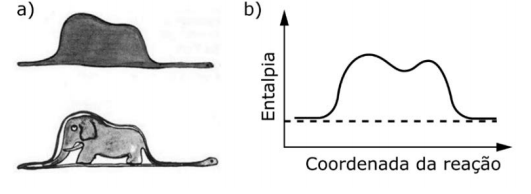
\includegraphics[width=.9\linewidth]{Fisico_Quimica/Termoquimica/figurab.jpg}
\end{center}


\begin{choice}
\choice Praticamente nula, com a formação de dois produtos.
\choice Altamente exotérmica, com a formação de dois produtos.
\choice Altamente exotérmica, mas nada se poderia afirmar sobre a quantidade de espécies no produto.
\choice Praticamente nula, mas nada se poderia afirmar sobre a quantidade de espécies no produto. 
\choice Nenhuma das alternativas.
\end{choice}
\end{exercise}
\begin{solution}
D
\end{solution}





\collectexercisesstop{TermoquimicaI}

%\printrandomexercises[collection=Balan,exclude=two]{8}
%\printrandomexercises[collection=TermoquimicaI,exclude=two]{8}


\collectexercises{RadioatividadeI}

\begin{exercise}[points=1.0]
\textbf{(PUC-SP)} O fenômeno da radioatividade foi descrito pela primeira vez no final do século passado, sendo largamente estudado no início do século XX. Aplicações desse fenômeno vão desde o diagnóstico e combate de doenças, até a obtenção de energia ou a fabricação de artefatos bélicos. Duas emissões radioativas típicas podem ser representadas pelas equações:

\begin{tblr}{c}
\isotope{238,U} \ch{->}  \isotope{234,Th} + $\upalpha$\\
\isotope{234,Th} \ch{->}  \isotope{234,Pa} + $\upbeta$
\end{tblr}


A radiação \(\upalpha\) é o núcleo do átomo de hélio, possuindo 2 prótons e 2 nêutrons, que se desprende do núcleo do átomo radioativo. A radiação \(\upbeta\) é um elétron, proveniente da quebra de um nêutron, formando também um próton, que permanece no núcleo. A equação que representa o decaimento radioativo do isótopo\isotope*{238,U} até o isótopo estável \isotope*{206,Pb} é:

\begin{choice}
\choice  \isotope*{238,U} \ch{->} \isotope*{206,Pb}  + \upalpha  \; + \upbeta.
\choice  \isotope*{238,U} \ch{->} \isotope*{206,Pb}  + 8\upalpha  \; + 4 \upbeta.
\choice  \isotope*{238,U} \ch{->} \isotope*{206,Pb}  + 8\upalpha \; + 6 \upbeta.
\choice \isotope*{238,U} \ch{->} \isotope*{206,Pb}  + 5\upalpha \; + 5 \upbeta.
\choice  \isotope*{238,U} \ch{->} \isotope*{206,Pb}  + 6\upalpha \; + 6 \upbeta.
\end{choice}
\end{exercise}
\begin{solution}
C
\end{solution}






\begin{exercise}[points=1.0]
Que mudanças ocorrem no número atômico e na massa de um núcleo durante cada um dos seguintes cenários de decaimento?
\begin{choice}
\choice uma partícula \(\alpha\) é emitida
\choice uma partícula \(\beta\) é emitida
\choice radiação \(\gamma\) é emitida
\choice um pósitron é emitido
\choice um elétron é capturado
\end{choice}
\end{exercise}
\begin{solution}
LETRA A
\end{solution}




\begin{exercise}[points=1.0]
O avanço científico e tecnológico da física nuclear permitiu conhecer, com maiores detalhes, o decaimento radioativo dos núcleos atômicos instáveis, desenvolvendo-se algumas aplicações para a radiação de grande penetração no corpo humano, utilizada, por exemplo, no tratamento do câncer. A aplicação citada no texto se refere a qual tipo de radiação?

\begin{choice}(2)
\choice Beta.
\choice Alfa.
\choice Gama.
\choice Raios X.
\choice Ultravioleta. 
\end{choice}
\end{exercise}
\begin{solution}
LETRA C
\end{solution}




\begin{exercise}[points=1.0]
Quem criou o primeiro reator nuclear?

\begin{choice}
\choice Albert Einstein
\choice Thomas Alva Edison
\choice Enrico Fermi
\choice Michael Faraday
\choice Enerst Rutherford
\end{choice}
\end{exercise}
\begin{solution}
LETRA C
\end{solution}



\begin{exercise}[points=1.0]
Alta energia de fotons emitidos são:

\begin{choice}
\choice Decaimento \(\alpha\)
\choice Decaimento \(\gamma\)
\choice Decaimento \(\beta\)
\choice Decaimento atômico
\choice Decaimento \(\Delta\)
\end{choice}
\end{exercise}
\begin{solution}
LETRA B
\end{solution}




\begin{exercise}[points=1.0]
A reação nuclear sofre o seguinte decaimento
\begin{reaction*}
\isotope{87,Br} ->  2 $\alpha$ + 3 $\beta$ + X
\end{reaction*}

Baseado nessa informação qual a configuração que o elemento X se apresenta

\begin{choice} (2)
\choice \ch{^{82}_{34}X}
\choice \ch{^{79}_{34}X}
\choice \ch{^{76}_{32}X}
\choice \ch{^{74}_{28}X}
\choice \ch{^{75}_{30}X}
\end{choice}
\end{exercise}

\begin{solution}
Letra B
\end{solution}


\begin{exercise}[points=1.0]
No decaimento do \isotope{238,U} ocorrem as seguintes transformações nucleares
\begin{reaction*}
\isotope{225,Ra} -> \isotope{214,Bi}
\end{reaction*}

Partindo do átomo de rádio até formar o átomo de bismuto, a sequência de emissões radiativas é:

\begin{choice}
\choice \(\alpha\), \(\alpha\), \(\alpha\), \(\upbeta\)
\choice \(\alpha, \upbeta, \upbeta, \upbeta\)
\choice \(\alpha, \upbeta, \alpha, \upbeta\)
\choice \(\upbeta, \alpha, \alpha, \upbeta\)
\choice \(\upbeta, \upbeta, \alpha, \alpha\)
\end{choice}
\end{exercise}
\begin{solution}
LETRA A
\end{solution}




\begin{exercise}[points=\PQ]
A partir da década de 40, quando McMillan e Seaborg obtiveram em laboratório os primeiros elementos transurânicos (NA > 92), o urânio natural foi usado algumas vezes para obter tais elementos. Para tanto, ele era bombardeado com núcleos de elementos leves. Na obtenção do Plutônio, do Califórnio e do Férmio as transmutações ocorreram da forma a seguir:

\begin{align*}
\isotope{U} + \isotope{He} \ch{->} \isotope{239,Pu} + A (\prescript{0}{1}{n})\\
\isotope{U} + \isotope{C} \ch{->} \isotope{245,Cf} + B (\prescript{0}{1}{n})\\
\isotope{U} + \isotope{12,O} \ch{->} \isotope{250,Fm} + C (\prescript{0}{1}{n})\\
\end{align*}

Sendo assim, os valores de A, B e C que indicam as quantidades de nêutrons obtidas são, respectivamente:

\begin{choice}(2)
\choice 1, 4 e 5.
\choice 1, 5 e 4.
\choice 2, 4 e 5.
\choice 3, 4 e 5.
\choice 3, 5 e 4.
\end{choice}
\end{exercise}
\begin{solution}
E
\end{solution}



\begin{exercise}[points=\PQ]
Um átomo X, de número atômico 92 e número de massa 238, emite uma partícula alfa, transformando-se num átomo Y, o qual emite uma partícula beta, produzindo um átomo Z. Então:

\begin{choice}(1)
\choice os átomos Y e X são isótopos.
\choice os átomos X e Z são isótonos.
\choice os átomos X e Y são isóbaros.
\choice o átomo Z possui 143 nêutrons.
\choice o átomo Y possui 92 prótons.
\end{choice}
\end{exercise}
\begin{solution}
D
\end{solution}



\begin{exercise}[points=\PQ]
A energia liberada durante a fissão nuclear pode ser utilizada para gerar eletricidade através da construção de usinas nucleares. Com base neste conhecimento, qual dos seguintes materiais é mais adequado para ser usado neste tipo de usina?


\begin{choice}(2)
\choice Ferro-56
\choice Neutrônio-0
\choice Uranio-235
\choice Hidrogênio-2
\choice Boro-10
\end{choice}
\end{exercise}
\begin{solution}
C
\end{solution}




\begin{exercise}[points=\PQ]
O processo da fissão nuclear pode ser iniciado por meio da absorção de um nêutron por parte do núcleo atômico, que é então dividido em dois fragmentos menores e mais estáveis, acompanhados pela liberação de outros nêutrons. Qual dos seguintes elementos químicos normalmente sofre fissão nuclear?

\begin{choice}(2)
\choice Urânio
\choice Hidrogênio
\choice Ferro
\choice Boro
\choice Cobalto
\end{choice}
\end{exercise}
\begin{solution}
A
\end{solution}



\begin{exercise}[points=\PQ]
As partículas alfa e beta possuem características físicas distintas e, por isso, apresentam comportamentos diferentes. A partícula alfa possui carga elétrica positiva, sendo formada por dois prótons e dois nêutrons. Já a partícula beta possui carga elétrica negativa ou positiva, dependendo do tipo de emissão. Qual dessas afirmativas está correta?

\begin{choice}(1)
\choice A partícula beta possui carga elétrica negativa e não possui massa.
\choice A partícula alfa possui carga elétrica negativa e é formada por dois prótons e dois nêutrons.
\choice A partícula alfa possui carga elétrica positiva e é formada por três prótons e três nêutrons.
\choice A partícula beta possui carga elétrica positiva e é formada por três prótons e três nêutrons.
\choice A partícula beta possui carga elétrica positiva e é formada por dois prótons e dois nêutrons.
\end{choice}
\end{exercise}
\begin{solution}
A
\end{solution}




\begin{exercise}[points=\PQ]
Atividade radioativa é o processo pelo qual um núcleo instável emite partículas e/ou radiação, em busca de estabilidade. Essa emissão de energia é conhecida como desintegração radioativa. O que acontece durante a desintegração radioativa?

\begin{choice}(1)
\choice O núcleo se desintegra totalmente.
\choice O núcleo transmuta para um elemento mais estável.
\choice O núcleo absorve energia.
\choice O núcleo se separa em duas partes.
\choice O núcleo se divide em três partes.
\end{choice}
\end{exercise}
\begin{solution}
B
\end{solution}


\begin{exercise}[points=\PQ]
Detectores de incêndio são dispositivos que disparam um alarme no início de um incêndio. Um tipo de detector contém uma quantidade mínima do elemento radioativo amerício-241. A radiação emitida ioniza o ar dentro e ao redor do detector, tornando-o condutor de eletricidade. Quando a fumaça entra no detector, o fluxo de corrente elétrica é bloqueado, disparando o alarme. Este elemento se desintegra de acordo com a equação a seguir:

\begin{reaction*}
\isotope{241,Am} -> \isotope{237,Np} + Z
\end{reaction*}

\begin{choice}(1)
\choice uma partícula alfa.
\choice uma partícula beta.
\choice radiação gama.
\choice raios X.
\choice dois prótons.
\end{choice}
\end{exercise}
\begin{solution}
A
\end{solution}


\begin{exercise}[points=\PQ]
Dadas as equações químicas:

\begin{enumerate}[label=\Roman*]
\item \ch{\isotope{239,Pu} -> $\upalpha$^4_{}2 + \isotope{235,U}}
\item \ch{\isotope{235,U} + {}^1_0n -> \isotope{91,Kr} + \isotope{142,Ba} + 3 ({}^1_0n)}
\item \ch{UF6_{\lqdd} -> UF6_{\gas}}
\end{enumerate}

Pode-se afirmar que ocorre fissão nuclear somente em:

\begin{choice}(2)
\choice I
\choice II
\choice III
\choice I e II
\choice I e III
\end{choice}
\end{exercise}
\begin{solution}
B
\end{solution}


\begin{exercise}[points=\PQ]
\textbf{(PUCCAMP)} O isótopo \isotope{131,I}, utilizado no diagnóstico de
moléstias da tireóide, pode ser obtido pelo bombardeio de \isotope{130,Te}, representado a seguir.

\begin{center}
\isotope{130,Te} + $_{1}^{0}${n} \ch{->} \isotope{131,I} + {\bfseries X}
\end{center}


Na equação radioquímica dada,  \textbf{X} corresponde a

\begin{choice}(2)
\choice próton
\choice nêutron
\choice pósitron
\choice partícula beta
\choice partícula alfa
\end{choice}
\end{exercise}
\begin{solution}
D
\end{solution}


\begin{exercise}[points=\PQ]
\textbf{(UEL)} Na transformação radioativa do \isotope{239,U} a \isotope{239,Pu} há emissão de:
\begin{choice}
\choice 2 partículas alfa.
\choice 2 partículas beta.
\choice 2 partículas alfa e 1 partícula beta.
\choice 1 partícula alfa e 2 partículas beta.
\choice 1 partícula alfa e 1 partícula beta.
\end{choice}
\end{exercise}
\begin{solution}
B
\end{solution}

\begin{exercise}[points=\PQ]
\textbf{(UEL)} Os elementos radiativos tem muitas aplicações. A seguir, estão exemplificadas algumas delas.

\begin{description}
\item[{I.}] O iodo é utilizado no diagnóstico de distúrbios da glândula tireóide, e pode ser obtido pela seguinte reação:
\end{description}
\begin{equation*}
\isotope{130,Te} \;  + \; _{0}^{1}n \rightarrow \isotope{153,I} + X
\end{equation*}
\begin{description}
\item[{II.}] O fósforo é utilizado na agricultura como elemento traçador para proporcionar a melhoria na produção do milho, e pode ser obtido pela reação:
\end{description}
\begin{equation*}
\isotope{35,Cl}\; +\; _{0}^{1}n \rightarrow \isotope{32,P} + Y
\end{equation*}
Sua reação de decaimento é: \isotope{32,P} \ch{->} \isotope{32,S} + Z
\begin{description}
\item[{III.}] O tecnécio é usado na obtenção de imagens do cérebro, fígado e rins, e pode ser representado pela reação:
\end{description}
\begin{equation*}
\isotope{99,Tc}  \rightarrow \isotope{99,Tc} + Q
\end{equation*}
Assinale a alternativa que indica, respectivamente, os significados de X, Y, Z e Q nas afirmativas I, II e III:

\begin{choice}(2)
\choice \upalpha, \upbeta, \upgamma, \upalpha
\choice \upalpha, \upbeta, \upalpha, \upgamma
\choice \upgamma, \upbeta, \upgamma, \upalpha
\choice \upbeta, \upalpha, \upbeta, \upbeta
\choice \upbeta, \upalpha, \upbeta, \upgamma
\end{choice}
\end{exercise}
\begin{solution}
E
\end{solution}



\collectexercisesstop{RadioatividadeI}


\collectexercises{RadioatividadeIOpen}



\begin{exercise}[points=1.0]


\begin{choice}(2)

\end{choice}
\end{exercise}
\begin{solution}
\end{solution}


\collectexercisesstop{RadioatividadeIOpen}
\collectexercises{RadioatividadeII-P2}

\begin{exercise}
A meia-vida de um isótopo radioativo é de 1,0 minuto. Em um experimento, o número de eventos de decaimento foi monitorado em 1-intervalos de minutos durante um período de 5 minutos. Suponha que 50 eventos de decaimento foram observados no primeiro minuto. No segundo minuto,\ldots{}\ldots{}. eventos foram observados, e no 5º minuto,\ldots{}.. eventos foram observados.
\begin{choice}
\choice 50, 50 
\choice 25, 3 
\choice  25, 25
\choice 50, 100
\choice 25, 13
\end{choice}
\end{exercise}
\begin{solution}
C
\end{solution}


\begin{exercise}
O urânio-238 decai para formar o tório-234 com meia-vida de \(4,5 \times 10^9\) anos. Quantos anos serão necessários para que 75\% da o urânio-238 decairá?
\begin{choice}
\choice \(9,0\times 10^{10}\)  anos 
\choice \(4,5 \times 10^9\) anos 
\choice \(4,5 \times 10^{10}\) anos
\choice \(9,0 \times 10^9\) anos
\choice \(3,8 \times 10^9\) anos
\end{choice}
\end{exercise}
\begin{solution}
B
\end{solution}


\begin{exercise}
Trítio, (\isotope{3,H}) é utilizado em placas luminosas de “SAÍDA” localizadas onde não há eletricidade para lâmpadas. Se a meia-vida de o trítio é 12,26 anos, que porcentagem da quantidade original do isótopo resta no sinal após 18,5 anos?
\begin{choice}
\choice 0.632\% 
\choice 63.2\% 
\choice 35.1\%
\choice 1.51\%
\choice 25.0\%
\end{choice}
\end{exercise}
\begin{solution}
D
\end{solution}

\begin{exercise}
O iodo-131 tem meia-vida de 8,1 dias e é usado como marcador da glândula tireóide. Se um paciente bebe um iodeto de sódio (NaI) contendo iodo-131 em uma terça-feira, quantos dias serão necessários para a concentração de iodo-131 atingir cair para 5,0\% de sua concentração inicial?
\begin{choice}
\choice 19 dias 
\choice 0,81 dia 
\choice 8,1 dias
\choice 35 dias 
\choice 25 dias
\end{choice}
\end{exercise}
\begin{solution}
D
\end{solution}

\begin{exercise}
O fósforo-32 é um isótopo radioativo usado como marcador no fígado. Quanto fósforo-32 foi originalmente usado se restam apenas 3,50 mg em uma amostra após 288 horas? (A meia-vida do fósforo-32 é de 14,3 dias.)
\begin{choice}
\choice 1,96 mg 
\choice 6,26 mg
\choice 4,17 mg
\choice 7,00mg
\choice 17,9mg
\end{choice}
\end{exercise}
\begin{solution}
B
\end{solution}


\begin{exercise}
As medições do carbono 14 nas embalagens de linho do Livro de Isaías nos Manuscritos do Mar Morto indicaram que os pergaminhos continham cerca de 79,5\% do carbono-14 encontrado nos tecidos vivos. Aproximadamente quantos anos têm esses pergaminhos? A meia-vida do carbono-14 é de 5.730 anos.

\begin{choice}
\choice 570 anos
\choice 1900 anos
\choice 820 anos
\choice 4600 anos
\choice 1300 anos
\end{choice}
\end{exercise}
\begin{solution}
B
\end{solution}


\collectexercisesstop{RadioatividadeII-P2}





\collectexercises{RadioatividadeII}

\begin{exercise}[points=1.0]
Considere o gráfico de decaimento, abaixo, ( Massa X Tempo ) de 12 g de um isótopo radioativo. Partindo - se de uma amostra de 80,0 g deste isótopo, em quanto tempo a massa dessa amostra se reduzirá a 20,0 g? Massa ( g )



\begin{tikzpicture}
		\begin{axis}[axis equal=false, grid=major,
			ylabel={\bfseries Massa (g)},
			xlabel={\bfseries Tempo (anos)}]
			\addplot[smooth,color=black,mark=*] coordinates {
			(0,12)
			(28,6)
			(56,3)
			(84,1.5)
			(112,0.75)
			%(100,3.125)
			};
		\end{axis}
\end{tikzpicture}

\begin{choice}(2)
\choice  112 anos
\choice 124,5 anos
\choice 84 anos
\choice 28 anos
\choice 56 anos
\end{choice}
\end{exercise}
\begin{solution}
E
\end{solution}




\begin{exercise}[points=1.0]
Qual é a meia-vida de um isótopo radioativo se uma amostra de 500,0g decai para 62,5g em 24,3 horas?

\begin{choice}(2)
\choice 8,1 horas
\choice 6,1 horas
\choice 12,15 horas
\choice 5 horas
\choice 24 horas
\end{choice}
\end{exercise}
\begin{solution}
LETRA A, 8,1 horas 
\end{solution}


\begin{exercise}[points=1.0]
O césio 137 é um isótopo radioativo produzido artificialmente. O gráfico a seguir indica a porcentagem desse isótopo em função do tempo


\begin{center}
\begin{tikzpicture}
	\begin{axis}[axis equal=false, grid=major,
		ylabel={\bfseries Massa de Césio -137},
		xlabel={\bfseries Tempo (anos)}]
		\addplot[smooth,color=black,mark=*] coordinates {
		(0,20)
		(30,10)
		(60,5)
		(90,2.5)
		(120,1.25)
		(150, 0.625)
		};
	\end{axis}
\end{tikzpicture}
\end{center}

Qual o tempo de meia vida da amostra?

\begin{choice}(2)
\choice 20 anos
\choice 40 anos
\choice 15 anos
\choice 25 anos
\choice 30 anos
\end{choice}
\end{exercise}
\begin{solution}
LETRA E 30 anos, pois corresponde a metade do tempo de meia vida
\end{solution}



\begin{exercise}[points=1.0]
Ao estudar a desintegração radioativa de um elemento, obteve-se uma meia-vida de 4h. Se a
massa inicial do elemento é 40g, depois de 12h, teremos (em gramas

\begin{choice}(2)
\choice 10
\choice 5
\choice 8
\choice 16
\choice 20
\end{choice}
\end{exercise}
\begin{solution}
B
\end{solution}


\begin{exercise}[points=1.0]
Têm-se 40g do isótopo \isotope{Na,24}. Sabendo-se que a meia-vida deste isótopo é igual a 15 horas,
depois de 75 horas, qual o percentual de massa radioativa restante?

\begin{choice}(2)
\choice 1,25\%
\choice 12,5\%
\choice 0,3125\%
\choice 31,25\%
\choice 3,125\%
\end{choice}
\end{exercise}
\begin{solution}
E
\end{solution}





\begin{exercise}[points=1.0]
O decaimento radioativo de uma amostra de césio - 137 está representado no gráfico a seguir


\begin{center}
\begin{tikzpicture}
		\begin{axis}[axis equal=false, grid=major,
			ylabel={\bfseries Massa de Césio -137},
			xlabel={\bfseries Tempo (anos)}]
			\addplot[smooth,color=black,mark=*] coordinates {
			(0,100)
			(20,50)
			(40,25)
			(60,12.5)
			(80,6.25)
			(100,3.125)
			};
		\end{axis}
\end{tikzpicture}
\end{center}

Tendo-se uma amostra com 80g de Cs-137, restarão apenas 5g desse radioisótopo após, aproximadamente:


\begin{choice}(2)
\choice 16 anos
\choice 30 anos
\choice 40 anos
\choice 80 anos
\choice 120 anos
\end{choice}
\end{exercise}
\begin{solution}
D
\end{solution}





\begin{exercise}[points=1.0]
Um ambiente foi contaminado com fósforo radioativo, \isotope{32,P}. A meia-vida desse radioisótopo é de 14 dias. A radioatividade por ele emitida deve cair a 12,5\% de seu valor original após:

\begin{choice}(2)
\choice 7 dias
\choice 14 dias
\choice 42 dias
\choice 51 dias
\choice 125 dias
\end{choice}
\end{exercise}
\begin{solution}
C
\end{solution}





\begin{exercise}[points=1.0]
O acidente do reator nuclear de Chernobyl, em 1986, lançou para a atmosfera grande quantidade de \isotope{90,Sr} radioativo, cuja meia-vida é de 28 anos. Supondo ser este isótopo a única contaminação radioativa e sabendo que o local poderá ser considerado seguro quando a quantidade de \isotope{90,Sr} se reduzir, por desintegração, a 1/16 da quantidade inicialmente presente, o local poderá ser habitado novamente a partir do ano de:

\begin{choice}(2)
\choice 2014
\choice 2098
\choice 2266
\choice 2986
\choice 3000
\end{choice}
\end{exercise}
\begin{solution}
A
\end{solution}





\begin{exercise}[points=1.0]
Uma certa massa inicial do radioisótopo trítio reduz-se a 200g em 36 anos. A mesma massa inicial leva 60 anos para se reduzir a 50g.
A meia-vida do trítio é igual a:


\begin{choice}(2)
\choice 60 anos
\choice 36 anos
\choice 30 anos
\choice 18 anos
\choice 12 anos
\end{choice}
\end{exercise}
\begin{solution}
E
\end{solution}





\begin{exercise}[points=1.0]
A meia-vida do isótopo \isotope{226,Ra} é igual a 2310 anos. Depois de quanto tempo a atividade de uma amostra desse isótopo radioativo se reduz de 75\% da atividade radioativa inicial?

\begin{choice}(2)
\choice 2310 anos.
\choice 4620 anos.
\choice 9200 anos.
\choice 6930 anos.
\choice 231 anos.
\end{choice}
\end{exercise}
\begin{solution}
B
\end{solution}





\begin{exercise}[points=1.0]
O lixo radioativo ou nuclear é resultado da manipulação de materiais radioativos, utilizados hoje na agricultura, na indústria, na medicina, em pesquisas científicas, na produção de energia, etc. Embora a radioatividade se reduza com o tempo, o processo de decaimento radioativo de alguns materiais pode levar milhões de anos. Por isso, existe a necessidade de se fazer um descarte adequado e controlado de resíduos dessa natureza. A taxa de decaimento radioativo é medida em termos de um tempo necessário para que uma amostra perca metade de sua radioatividade original. O gráfico seguinte representa a taxa de decaimento radioativo do rádio – 226, elemento químico pertencente à família dos metais alcalinoterrosos e que foi utilizado durante muito tempo na medicina.

\begin{center}
\begin{tikzpicture}
	\begin{axis}[
	%	width=10cm,height=7cm,
		%grid=both,
		%	enlargelimits=true,
		%scale only axis,
		axis x line =middle,
	    axis y line = middle,
		inner axis line style={=>},
	%	domain = 2:12,
	%	samples = 11,
		xlabel={Anos},
		%ylabel={kg},
		ymin=0,
		xmin=0,
		xlabel style={yshift=-10mm,},
		ylabel style={xshift=-12mm,},
		%yticklabel={$\pgfmathprintnumber{\tick}/{2}$},
		%yticklabel={1, $\frac{1}{2}$}
		xtick = {0, 1620, 3240, 4860},
	%	ytick = {1,4, 2, 1},
		ytick = {100,50, 25, 12.5},
	%	yticklabel={$\pgfmathprintnumber{\tick}$\%}
		yticklabels={1 kg, $\sfrac{1}{2}$ kg,$\sfrac{1}{4}$ kg, $\sfrac{1}{8}$ kg},
		ymax=120,
		xmax=6480
		]
		\addplot+[black,smooth] coordinates {
		(00,100) (1620,50) (3240,25) (4860,12.5)
		};
		\draw[dashed](163,0)--(163,50);
		\draw[dashed](163,50)--(0,50);
		\draw[dashed](325,0)--(325,25);
		\draw[dashed](325,25)--(0,25);
		\draw[dashed](485,0)--(485,12.5);
		\draw[dashed](485,12.5)--(0,12.5);
		\draw (55,105)  node[minimum size=0.5cm,draw,fill=gray] {};
		%\draw (195,56)  node[minimum size=0.5cm,draw] {};
		\draw[path picture={\fill[gray] (path picture bounding box.south west)
			rectangle (path picture bounding box.east);}] (180,51) rectangle  ++ (37,11);
		%\draw (378,29)  node[minimum size=0.5cm,draw] {};
%		\draw (378,27)  node[minimum height=0cm,minimum width=0.5cm,draw,fill=red] {};
		 %\draw (378,27)	node[text width=0.3cm,text height=0.05cm,fill=green]{};
		 \draw[draw] (357,24) rectangle  ++ (39,11);
		 \draw[draw,fill=gray] (357,24) rectangle  ++ (39,3);
		 \draw[draw] (502,10) rectangle  ++ (39,11);
		 \draw[draw,fill=gray] (502,10) rectangle  ++ (39,1);
		\end{axis}
\end{tikzpicture}
\end{center}

As informações fornecidas mostram que:



\begin{choice}(1)
\choice Quanto maior a meia-vida de uma substância, mais rápido ela se desintegra.
\choice Apenas 1/8 de uma amostra de rádio – 226 terá decaído ao final de 4860 anos.
\choice Metade da quantidade original de rádio – 226, ao final de 3240 anos, ainda estará por decair.
\choice Restará menos de 1\% de rádio – 226 em qualquer amostra dessa substância após decorridas 3 meias-vidas.
\choice A amostra de rádio – 226 diminui a sua quantidade pela metade a cada intervalo de 1620 anos devido à desintegração radioativa.
\end{choice}
\end{exercise}
\begin{solution}
E
\end{solution}





\begin{exercise}[points=1.0]
Considere os seguintes materiais:

\begin{enumerate}[label=\Roman*]
\item Artefato de bronze (confeccionado pela civilização inca).
\item Mangueira centenária (que ainda produz frutos nas ruas de Belém do Pará).
\item Corpo humano mumificado (encontrado em tumbas do Egito antigo).
\end{enumerate}

O processo de datação, por carbono -14, é adequado para estimar a idade apenas:

\begin{choice}(1)
\choice do material I.
\choice do material II.
\choice do material III.
\choice dos materiais I e II.
\choice do material II e III.
\end{choice}
\end{exercise}
\begin{solution}
C
\end{solution}




\begin{exercise}[points=1.0]
Um isótopo radioativo de tálio (Tl) emite partícula beta e se transforma em chumbo (Pb) estável. A meiavida desse isótopo é 3,1 minutos. Partindo-se de uma amostra de Tl puro, verifica-se a presença de 7 gramas de Pb nessa amostra depois de 9,3 minutos. A massa de Tl na amostra Inicial era:

\begin{choice}(2)
\choice 7 g
\choice 8 g
\choice 14 g
\choice 28 g
\choice 56 g
\end{choice}
\end{exercise}
\begin{solution}
B

Em 9,3 s se passaram 3 meias-vidas e por isso só restam 12,5\% da massa original de Talio.Consequentemente 87,5 \% da massa original de Tálio se transformou em chumbo.
7g------------------87,5\%
xg-----------------100\%
x=700/87,5
x=8g de Tálio(massa inicial)
\end{solution}





\begin{exercise}[points=1.0]
A meia-vida do rádio é 1620 anos. Que porcentagem aproximada de uma dada quantidade de rádio estará desintegrada após 162 anos?

\begin{choice}(2)
\choice 6,7\%
\choice 20,1\%
\choice 33,5\%
\choice 93,3\%
\choice 100\% 
\end{choice}
\end{exercise}
\begin{solution}
A
\end{solution}





\begin{exercise}[points=1.0]
O isótopo radioativo Cu-64 sofre decaimento \(\upbeta\), conforme representado:

\begin{reaction*}
\isotope{64,Cu} ->  \isotope{64,Zn} + {}_{-1}^0\upbeta
\end{reaction*}

A partir de amostra de 20,0 mg de Cu-64, observa-se que, após 39 horas, formaram-se 17,5 mg de Zn-64. Sendo assim, o tempo necessário para que metade da massa inicial de Cu-64 sofra decaimento \(\upbeta\) é cerca de


\begin{choice}(2)
\choice 6 horas.
\choice 13 horas.
\choice 19 horas.
\choice 26 horas.
\choice 52 horas.
\end{choice}
\end{exercise}
\begin{solution}
B
\end{solution}





\begin{exercise}[points=1.0]
Um radioisótopo, para ser adequado para fins terapêuticos, deve possuir algumas qualidades, tais como: emitir radiação gama (alto poder de penetração) e meia-vida apropriada. Um dos isótopos usados é o tecnécio-99, que emite este tipo de radiação e apresenta meia-vida de 6 horas. Qual o tempo necessário para diminuir a emissão dessa radiação para 3,125 \% da intensidade inicial?

\begin{choice}(2)
\choice 12 horas.
\choice 18 horas.
\choice 24 horas.
\choice 30 horas.
\choice 36 horas
\end{choice}
\end{exercise}
\begin{solution}
D
\end{solution}





\begin{exercise}[points=1.0]
De vilão a mocinho! Assim pode ser considerado o fenômeno da radioatividade. As radiações podem causar sérios danos biológicos. Produzem e são causadoras de leucemia e de câncer. Entretanto, em doses controladas, a radiação é utilizada para combater e, em alguns casos, eliminar essas doenças. Considerando-se a cinética das emissões radioativas, se a massa de um isótopo radioativo se reduz a 12,5\% do valor inicial depois de um ano, e considerando-se que um ano tem exatamente 12 meses, então a meiavida desse isótopo, em meses, é:

\begin{choice}(2)
\choice 8
\choice 6
\choice 4
\choice 3
\choice 2
\end{choice}
\end{exercise}
\begin{solution}
C
\end{solution}




\begin{exercise}[points=1.0]
Por meio de estudos pormenorizados realizados por bioantropólogos mexicanos, constatou-se que as feições do fóssil humano mais antigo já encontrado no México eram muito parecidas com aborígines australianos. O fóssil em questão, com 12 mil anos, é o crânio conhecido como Mulher de Penón. A determinação da idade de um fóssil é baseada no decaimento radioativo do isótopo carbono-14, cujo tempo de meia vida é de aproximadamente 6000 anos. A percentagem de carbono-14 encontrada atualmente no fóssil em relação àquela contida no momento da morte é aproximadamente igual a:

\begin{choice}(2)
\choice 25 \%
\choice 37 \%
\choice 50 \%
\choice 75 \%
\choice 90 \%
\end{choice}
\end{exercise}
\begin{solution}
A
\end{solution}





\begin{exercise}[points=1.0]
Qual o tempo necessário para que um elemento radioativo tenha sua massa diminuída em 96,875\%?

\begin{choice}(2)
\choice 3 meias-vidas.
\choice 10 vidas-médias.
\choice 5 meias-vidas.
\choice 96,875 anos.
\choice 312 anos.
\end{choice}
\end{exercise}
\begin{solution}
C
\end{solution}





\begin{exercise}[points=1.0]
Na conferência de 1998, a Sociedade Nuclear Europeia mostrou muita preocupação acerca do perigo do lixo nuclear. Por exemplo, a desintegração do isótopo \isotope{90,Sr}, um dos elementos mais nocivos à vida, se dá através de emissões beta (\(\upbeta\) ) de elevada energia, cuja meia-vida é de 28 anos. Considerando uma massa inicial de 24 mg desse isótopo, a massa aproximada em miligramas, após 100 anos, será:

\begin{choice}(2)
\choice 1,0
\choice 2,0
\choice 4,0
\choice 8,0
\choice 16
\end{choice}
\end{exercise}
\begin{solution}
B
\end{solution}





\begin{exercise}[points=1.0]
Um elemento radioativo com Z = 53 e A = 131 emite partículas alfa e beta, perdendo 75\% de sua atividade em 32 dias. Detemine o tempo de meia-vida deste radioisótopo

\begin{choice}(2)
\choice 8 dias
\choice 16 dias
\choice 5 dias
\choice 4 dias
\choice 2 dias
\end{choice}
\end{exercise}
\begin{solution}
B
\end{solution}


\begin{exercise}[points=\PQ]
\textbf{(ENEM)} Glicose marcada com nuclídeos de carbono-11 é utilizada na medicina para se obter imagens tridimensionais do cérebro, por meio de tomografia de emissão de pósitrons. A desintegração do carbono-11 gera um pósitron, com tempo de meia-vida de 20,4 min, de acordo com a equação da reação nuclear:
\begin{reactions*}
\isotope{11,C} -> \isotope{11,B} + e_{0}^1
\end{reactions*}

A partir da injeção de glicose marcada com esse nuclídeo, o tempo de aquisição de uma imagem de tomografia é de \textbf{cinco meias-vidas}. Considerando que o medicamento contém 1,00 g do carbono-11, a massa, em miligramas (mg), do nuclídeo restante, após a aquisição da imagem, é mais próxima de

\begin{choice}(2)
\choice 0,5.
\choice 0,25.
\choice 0,0625.
\choice 200.
\choice 31,3.
\end{choice}
\end{exercise}
\begin{solution}
LETRA E
\end{solution}




\begin{exercise}[points=\PQ]
\textbf{(UFSCAR)} Em 1999, foi estudada a ossada do habitante considerado mais antigo do Brasil, uma mulher que a equipe responsável pela pesquisa convencionou chamar Luzia. A idade da ossada foi determinada como sendo igual a 11.500 anos. Suponha que, nesta determinação, foi
empregado o método de dosagem do isótopo radioativo carbono-14, cujo tempo de meia-vida é de 5.730 anos. Pode-se afirmar que a quantidade de carbono-14
encontrada atualmente na ossada, comparada com a contida no corpo de Luzia por ocasião de sua morte, é aproximadamente igual a
\begin{choice}
\choice 100\% do valor original.
\choice 50\% do valor original.
\choice 25\% do valor original.
\choice 10\% do valor original.
\choice 5\% do valor original.
\end{choice}
\end{exercise}
\begin{solution}
C
\end{solution}


\begin{exercise}[points=\PQ]
\textbf{(ENEM)} A duração do efeito de alguns fármacos está relacionada à sua meiavida, tempo necessário para que a quantidade original do fármaco no organismo se reduza à metade. A cada intervalo de tempo correspondente a uma meiavida, a quantidade de fármaco existente no organismo no final do intervalo é igual a 50\% da quantidade no início desse intervalo.
O gráfico acima representa, de forma genérica, o que acontece com a quantidade de fármaco no organismo humano ao longo do tempo.

\emph{ {\scriptsize F. D. Fuchs e Cher l. Wannma. Farmacologia Clínica. Rio de Janeiro: Guanabara Koogan,1992, p. 40.}}

\begin{center}
\begin{tikzpicture}
		\begin{axis}[axis equal=false, grid=major,
			ylabel={\bfseries \% de fármaco no organismo},
			xlabel={\bfseries números de meias-vidas}]
			\addplot[smooth,color=black,mark=*] coordinates {
			(0,100)
			(1,50)
			(2,25)
			(3,12.5)
			(4,6.25)
			(5,3.125)
                        (6,1.5625)
                        (7,0.78125)
                        (8,0.390625)
			};
		\end{axis}
\end{tikzpicture}
\end{center}

A meia-vida do antibiótico amoxicilina é de 1 hora. Assim, se uma dose desse antibiótico for injetada às 12 h em um paciente, o percentual dessa dose que restará em seu organismo às 13 h 30 min será aproximadamente de

\begin{choice}(2)
\choice 10\%.
\choice 15\%.
\choice 25\%.
\choice 35\%.
\choice 50\%.
\end{choice}
\end{exercise}
\begin{solution}
D
\end{solution}












\collectexercisesstop{RadioatividadeII}


\collectexercises{RadioatividadeIIOpen}

\begin{exercise}[points=\PQA]
Glenn T. Seaborg é um renomado cientista que foi agraciado com o Prêmio Nobel de Química em 1951, por seus trabalhos em radioquímica. Em 1974 foi sintetizado, nos Estados Unidos, o elemento de número atômico 106 que, em sua homenagem, teve como nome proposto Seaborgium (\isotope{Sg}).

\begin{choice}
\choice O bombardeio do \isotope{249,Cf} por um elemento X produz o \isotope{263,Sg} e 4 nêutrons. Determine o número atômico e o número de massa do elemento X.



\blank[blank-style={\phantom{#1}},width=3\linewidth]{}


\choice Sabendo que um determinado isótopo do \isotope{106,Sg} perde 50\% de sua massa inicial em 10 segundos, calcule a massa final de uma amostra de 800 gramas deste isótopo após 30 segundos.
\end{choice}


\blank[blank-style={\phantom{#1}},width=8\linewidth]{}
\end{exercise}
\begin{solution}



a) Massa atômica= 18

Prótons= 8

249\textsuperscript{Cf}\textsubscript{98} + b\textsuperscript{X}\textsubscript{a} ---------------> 263\textsuperscript{Sg}\textsubscript{106} + 4 1\textsuperscript{n}\textsubscript{0}

249 + b = 263 +4

b= 18

98 + a = 106

a = 8


b)


b) Xfinal = X0 * (1/2)\textsuperscript{tempo}/meia vida

Xfinal = 800* (1/2)\textsuperscript{30}/10

Xfinal= 100g            OU

800g ------- 10 s -----> 400g ---- 10s ----> 200g --- 10s ---> 100g
\end{solution}



\begin{exercise}[points=\PQA]
A Tomografia PET permite obter imagens do corpo humano com maiores detalhes, e menor exposição à radiação, do que as técnicas tomográficas atualmente em uso. A técnica PET utiliza compostos marcados com \isotope{11,C}. Este isótopo emite um pósitron, \(_{+1}e^0\), formando um novo núcleo, em um processo com tempo de meia-vida de 20,4 minutos. O pósitron emitido captura rapidamente um elétron, \(_1e^0\), e se aniquila, emitindo energia na forma de radiação gama.

\begin{choice}
\choice Escreva a equação nuclear balanceada que representa a reação que leva à emissão do pósitron. O núcleo formado no processo é do elemento B(Z=5), C(Z=6), N(Z=7) ou O(Z=8)?


\blank[blank-style={\phantom{#1}},width=8\linewidth]{}



\choice  Determine por quanto tempo uma amostra de \isotope{11,C} pode ser usada, até que sua atividade radioativa se reduza a 25\% de seu valor inicial.


\blank[blank-style={\phantom{#1}},width=8\linewidth]{}
\end{choice}
\end{exercise}


\begin{exercise}[points=\PQA]
Para diagnósticos de anomalias da glândula tireóide, por cintilografia, deve ser introduzido, no paciente, iodeto de sódio, em que o ânion iodeto é proveniente de um radioisótopo do iodo (número atômico 53 e número de massa 131). A meia-vida efetiva desse isótopo (tempo que decorre para que metade da quantidade do isótopo deixe de estar presente na glândula) é de aproximadamente 5 dias.

\begin{choice}
\choice O radioisótopo em questão emite radiação  $_{-1}^{0}\upbeta$  . O elemento formado nessa emissão é \isotope{131,Xe}? Justifique. Escreva a equação nuclear correspondente.


\blank[blank-style={\phantom{#1}},width=8\linewidth]{}

\choice Suponha que a quantidade inicial do isótopo na glândula (no tempo zero) seja de 1,000 g e se reduza, após certo tempo, para 0,125 g. Com base nessas informações, trace a curva que dá a quantidade do radioisótopo na glândula em função do tempo, colocando os valores nas coordenadas adequadamente escolhidas.
\end{choice}


\begin{tikzpicture}
	\begin{axis}[grid=both, ticks=none,axis x line=bottom,axis y line=left
			,]
\end{axis}
\end{tikzpicture}
\end{exercise}






\begin{exercise}[points=\PQA]
A bomba atômica se baseia na fissão de núcleos pesados, formando dois núcleos mais leves. O urânio-235 pode sofrer fissão de acordo com a equação:
\begin{equation*}
\prescript{}{92}{\mathrm{U}}^{235} + \prescript{}{0}{\mathrm{n}}^1 \ch{->} \prescript{}{38}{\mathrm{Sr}}^{94} + \prescript{}{Z}{\mathrm{X}^A} + 3 \prescript{}{0}{\mathrm{n}}^1
\end{equation*}

Qual o número de nêutrons do nuclídeo \(\prescript{}{Z}{\mathrm{X}^A}\)

\blank[blank-style={\phantom{#1}},width=8\linewidth]{}
\end{exercise}




\begin{exercise}[points=\PQA]
Recentemente, a imprensa noticiou o caso do envenenamento por polônio-210 de um exagente secreto soviético. Sabe-se, em relação a esse isótopo, que:

\begin{itemize}
\item ao se desintegrar, emite uma partícula alfa;
\item em 420 dias, uma amostra de 200 mg decai para 25 mg;
\item o isótopo formado nesse decaimento forma um íon divalente.
\end{itemize}

Calcule o tempo de meia-vida do polônio-210.

\blank[blank-style={\phantom{#1}},width=8\linewidth]{}
\end{exercise}


\begin{exercise}[points=\PQA]
"(\ldots{}) A Mir está deixando os cientistas intrigados: minúsculas partículas de urânio empobrecido foram detectadas na estação. Três hipóteses foram levantadas pela equipe de pesquisadores: o urânio seria de armas nucleares testadas no espaço na década de 60, restos de satélites, ou vestígios de uma supernova. (\ldots{}) Foram descobertos sinais de dois isótopos radioativos - \isotope{214,Pb} e \isotope{214,Bi} - ambos resultantes do \isotope{238,U}"

(JB, 2001).
.

Considerando que a meia-vida do \isotope{214,Bi} é de 20 meses calcule, a partir de uma amostra com 1,000 g de \isotope{214,Bi}, quantos miligramas restarão depois de 5 anos? 



\blank[blank-style={\phantom{#1}},width=8\linewidth]{}
\end{exercise}
\begin{solution}
125 mg
\end{solution}


\collectexercisesstop{RadioatividadeIIOpen}


%\printrandomexercises[collection=RadioatividadeI,exclude=four]{4}
%\printrandomexercises[collection=RadioatividadeII,exclude=four]{4}
%\printrandomexercises[collection=RadioatividadeIIOpen]{1}
\end{document}
